\documentclass[11pt, a4paper]{article}
\usepackage[table,xcdraw]{xcolor}
\usepackage[portuges]{babel}
\usepackage[utf8]{inputenc}
\usepackage{graphicx}
\usepackage{float}
\usepackage{indentfirst}
\usepackage{hyperref}
\usepackage{multirow}
\usepackage[table,xcdraw]{xcolor}
\usepackage{longtable}
\usepackage[toc, title]{appendix}
\usepackage{a4wide}
\usepackage{array}
\usepackage{enumitem}
\usepackage{amssymb}
\usepackage{pifont}
\usepackage{makecell}
\usepackage{subfig}
\usepackage{bookmark}

\newcommand{\xmark}{\ding{55}}

\begin{document}

\setcounter{tocdepth}{4}
\setcounter{secnumdepth}{4}
\begin{titlepage}

\newcommand{\HRule}{\rule{\linewidth}{0.5mm}} % Defines a new command for the horizontal lines, change thickness here

\center % Center everything on the page

\begin{figure}[H]
    \centering
    
\includegraphics[scale=0.5]{images/UM_EENG.jpg}
    \label{figUM}
\end{figure}

\large Universidade do Minho\\[0.2cm] % Name of your university/college
\large Mestrado Integrado em Engenharia Informática\\[0.2cm] % Major heading such as course 
\large Departamento de Informática\\[2.5cm] % Major heading such as course name

\textsc{\Large Projeto em Engenharia Informática}\\[0.3cm] % Minor heading such as course title
\HRule \\[0.3cm]
{ \LARGE \bfseries Automação Robótica de Processos (RPA) usando um chatbot Telegram}\\[0.4cm] % Title of your document
{ \LARGE \bfseries Testes de Usabilidade}\\[0.3cm]
\HRule \\[0.3cm]

\begin{figure}[H]
    \centering
    
\includegraphics[scale=0.6]{images/nos.png}
    \label{figNOS}
\end{figure}

% [2.5cm]

{\large Ano Letivo de 2019/2020}\\ % Date, change the \today to a set date if you want to be precise

\vspace*{\fill}
\noindent
{\large \textbf{Grupo i1}}\\[0.5cm]
Fábio Gonçalves \textsc{A78793}\\[0.3cm]
Francisco Oliveira \textsc{A78416}\\[0.3cm]
Gonçalo Camaz \textsc{A76861}\\[0.3cm]
João Vieira \textsc{A78468}\\[0.3cm]
José Carlos Martins \textsc{A78821}\\[0.3cm]
Miguel Quaresma \textsc{A77049}\\[0.3cm]
Raul Vilas Boas \textsc{A79617}\\[0.3cm]
Salete Teixeira \textsc{A75281}\\[0.3cm]
Simão Barbosa \textsc{A77689}

\end{titlepage}

\newpage

\thispagestyle{empty}
\setcounter{page}{0}
\tableofcontents
\clearpage

\newpage

\section{Testes de usabilidade}
A realização de testes de usabilidade com o intuito de aferir a facilidade de interação e utilidade de um dado sistema (em desenvolvimento), representa uma componente fundamental do ciclo de desenvolvimento visto que permite determinar falhas no sistema tanto a nível de funcionamento como de UX (\textit{User eXperience}). Ao integrar estes testes em diversas fases do ciclo de desenvolvimento é possível ajustar o sistema de maneira iterativa com base no \textit{feedback} resultante dos mesmos.

O sistema desenvolvido apresenta, no entanto, particularidades que influenciam os aspectos passíveis de serem alvo dos testes de usabilidade, nomeadamente a ausência de \textit{interface}, que é da responsabilidade do serviço de \textit{messaging} utilizado. Nesse sentido o sistema será avaliado nestes testes com base em critérios como a velocidade de resposta, a estrutura e correção da resposta e o número de funcionalidades disponibilizadas.

\section{Testes com Protótipo do ChatBot}
Numa fase inicial, e com o intuito de validar previamente o sistema a desenvolver, foram realizados testes
simulados que recorreram a um Bot determinístico, com respostas criadas com o intuito de emular o
comportamento esperado do sistema. Adicionalmente, foi definido um conjunto de perguntas predefinidas que
seriam realizadas pelos utilizadores que constituíram a amostra. Nestes testes, a interacção dos
utilizadores com o sistema foi feita através do \textit{Telegram}, para permitir a obtenção de
\textit{feedback} quanto à estrutura das respostas apresentadas pelo sistema.  A realização destes testes
visou duas das quatro componentes do sistema, Cinema Webscraper e FS Webscraper, pretendendo com isto testar
a capacidade de resposta de cada um destes micro-serviços e recolher dados que permitissem melhorar o sistema
de processamento de linguagem natural usado pela componente Chat Processor.

\subsection{Amostra da População}
Com o objetivo de averiguar o funcionamento do sistema em cenários reais, o grupo realizou testes de usabilidade com utilizadores sem conhecimentos relativos ao projeto desenvolvido. 
Para simular a utilização do sistema, o grupo selecionou um público alvo com o intuito de analisar a interação do mesmo com a sistema e perceber quais eram as principais dificuldades dos utilizadores. 
Nesta secção vamos especificar a amostragem da população selecionada e discutir os resultados obtidos com os testes de usabilidade, apresentando o feedback recebido por parte dos utilizadores.
O sistema, quando aplicado num cenário real pode atingir diversos utilizadores com grande diferença de idades. Para além desse factor, é de extrema 
importância o grau de conhecimento que cada utilizador possui relativamente à interacção com equipamentos como um telemóvel ou um computador, dado que
este influencia directamente os aspectos positivos e negativos apontados por cada utilizador.

Na tabela seguinte é possível observar os diversos membros da população abordada com as respectivas idades, género, níveis de conhecimento na área da tecnologia e frequência de interação com a mesma.


\begin{longtable}[c]{|c|c|c|}
\hline
ID & Idade &  Conhecimento \\ \hline
1 & 28  & \begin{tabular}[c]{@{}c@{}}Utilizador que utiliza com frequência \\ tecnologias e que possui conhecimento sobre \\ as mesmas\end{tabular} \\ \hline
2 & 34  & \begin{tabular}[c]{@{}c@{}}Utilizador que utiliza com frequência\\ tecnologias mas com pouco conhecimento\\ sobre as mesmas\end{tabular} \\ \hline
3 & 54 & \begin{tabular}[c]{@{}c@{}}Utilizador com baixo conhecimento na \\ área da tecnologia e com baixa frequência\\ de utilização\end{tabular} \\ \hline
4 & 55 & \begin{tabular}[c]{@{}c@{}}Utilizador que utiliza com frequência\\ tecnologias mas com pouco conhecimento\\ sobre as mesmas\end{tabular} \\ \hline
5 & 28 & \begin{tabular}[c]{@{}c@{}}Utilizador que utiliza com frequência \\ tecnologias e que possui conhecimento sobre \\ as mesmas\end{tabular} \\ \hline
6 & 22 & \begin{tabular}[c]{@{}c@{}}Utilizador que utiliza com frequência\\ tecnologias mas com pouco conhecimento\\ sobre as mesmas\end{tabular} \\ \hline
7 & 50 & \begin{tabular}[c]{@{}c@{}}Utilizador com baixo conhecimento na \\ área da tecnologia e com baixa frequência\\ de utilização\end{tabular} \\ \hline
8 & 55 & \begin{tabular}[c]{@{}c@{}}Utilizador com baixo conhecimento na \\ área da tecnologia e com baixa frequência\\ de utilização\end{tabular} \\ \hline
9 & 23 & \begin{tabular}[c]{@{}c@{}}Utilizador que utiliza com frequência\\ tecnologias mas com pouco conhecimento\\ sobre as mesmas\end{tabular} \\ \hline
10 & 14 & \begin{tabular}[c]{@{}c@{}}Utilizador que utiliza com frequência\\ tecnologias mas com pouco conhecimento\\ sobre as mesmas\end{tabular} \\ \hline
11 & 50 & \begin{tabular}[c]{@{}c@{}}Utilizador que utiliza com frequência\\ tecnologias mas com pouco conhecimento\\ sobre as mesmas\end{tabular} \\ \hline
12 & 49 & \begin{tabular}[c]{@{}c@{}}Utilizador que utiliza com frequência\\ tecnologias e possui elevado conhecimento\\ sobre as mesmas\end{tabular} \\ \hline
13 & 33 & \begin{tabular}[c]{@{}c@{}}Utilizador com baixo conhecimento na \\ área da tecnologia e com baixa frequência\\ de utilização\end{tabular} \\ \hline
14 & 34 & \begin{tabular}[c]{@{}c@{}}Utilizador que utiliza com frequência\\ tecnologias mas com pouco conhecimento\\ sobre as mesmas\end{tabular} \\ \hline
\caption{Amostragem da população abordada nos testes de usabilidade}
\label{tab:my-table}\\
\end{longtable}

Na figura abaixo é possível observar o intervalo de idades da população na amostra recolhida. É possível verificar que foi realizado um número superior de testes em utilizadores com idades compreendidas entre os 20 e os 39, e entre os 50 e 60 anos. 

\begin{figure}[H]
    \centering
    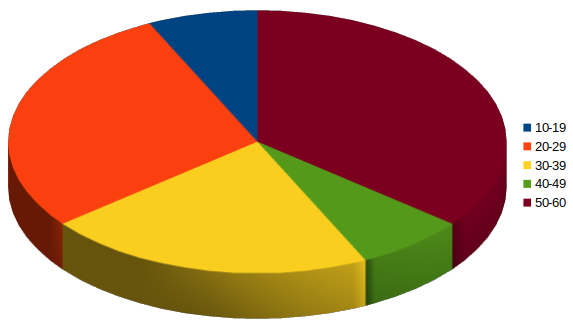
\includegraphics[scale=0.5]{images/idades.png}
    \label{figIdades}
    \caption{Idades da amostragem}
\end{figure}

O nível de conhecimento na área da tecnologia da maioria da população da amostragem é reduzido.
Assim será possível perceber se o nosso sistema é de fácil utilização, mesmo quando o utilizador não possui conhecimentos na área.
\begin{figure}[H]
    \centering
    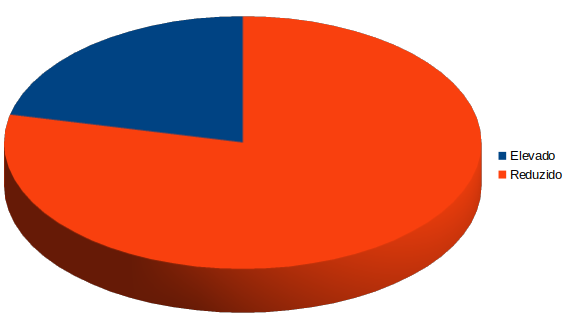
\includegraphics[scale=0.5]{images/conhecimento.png}
    \label{figConhecimentos}
    \caption{Nível de conhecimento na área da tecnologia da amostragem}
\end{figure}

A frequência de interação com tecnologia como telemóveis e computadores tem um papel importante, visto que, um utilizador com utilização frequente tem tendência para conseguir interagir com o sistema de uma forma mais fluída. 
\begin{figure}[H]
    \centering
    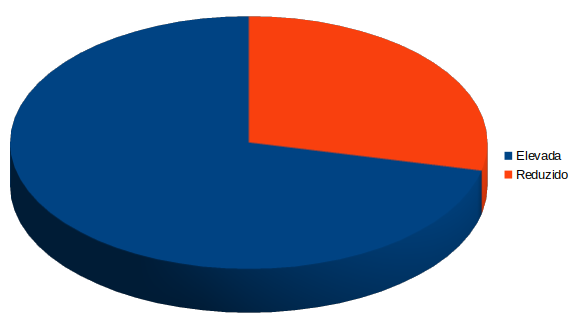
\includegraphics[scale=0.5]{images/frequenciautilizacao.png}
    \label{figFrequencia}
    \caption{Frequência de interação com tecnologia}
\end{figure}


\subsection{Metodologia de testes}
A realização de testes de usabilidade em sistemas complexos pressupõe a escolha de um
conjunto de funcionalidades que deverão ser alvo destes testes. Estas funcionalidades devem ser compreensivas
o suficiente para que os resultados dos testes permitam obter uma visão geral do sistema sem que seja necessário
testar todas as suas vertentes. Nesse sentido, para os testes de usabilidade com o protótipo do sistema, foram
escolhidas, com alvo dos testes, as seguintes funcionalidades:

\begin{itemize}
    \item Cinema Webscraper
        \begin{enumerate}
            \item Cinemas por proximidade.
            \item Cinemas numa determinada cidade.
            \item Filmes em exibição por cidade.
            \item Filmes com um determinado ator.
            \item Próximas estreias.
            \item Próximas sessões.
            \item Próximas sessões de um determinado filme.
        \end{enumerate}
    \item FS Webscraper
        \begin{enumerate}
            \setcounter{enumi}{7}
            \item Linha de apoio para pacotes da NOS.
            \item Informações sobre um telemóvel em específico.
            \item Telemóveis que se encontram em promoção.
            \item Tarifários WTF.
            \item Pacotes fibra por limite de preço.
            \item Pacotes satélite com um determinado serviço.
            \item Lojas NOS numa determinada cidade.
        \end{enumerate}
\end{itemize}

Para além de permitir averiguar a qualidade das respostas do sistema, os testes realizados permitiram
ainda a recolha de dados linguísticos relativos à interação dos utilizadores, que foram usados para melhorar
a capacidade de processamento de linguagem natural do mesmo.

\subsection{Resultados agregados dos utilizadores}

O \textit{feedback} recolhido nos testes de usabilidade encontra-se agregado, por funcionalidade, na tabela
seguinte:

\begin{longtable}{|c|m{12cm}|c|}
        \hline
        Pergunta & Sugestões & Feito? \\ \hline
        1 & \begin{itemize}[leftmargin=0.5cm]
            \setlength\itemsep{0em}
            \item Enumerações com ``-'' ou ``*'' para melhor apresentação.
            \item Indicar se o cinema tem boas acessibilidades.
            \item Informação da localidade, ou \textit{link} para o \textit{Google Maps}.
            \item Categorizar cinemas por distância.
        \end{itemize} &
        \makecell{
            \textcolor{green}{\checkmark} \\[0.4em]
            \textcolor{red}{\xmark} \\[0.4em]
            \textcolor{red}{\xmark} \\[0.4em]
            \textcolor{red}{\xmark}
        }\\ \hline
        
        2 & \begin{itemize}[leftmargin=0.5cm]
            \setlength\itemsep{0em}
            \item Enumerações com ``-'' ou ``*'' para melhor apresentação.
            \item Indicar o cinema que está mais perto de ``mim''.
            \item Informação da localidade, ou \textit{link} para o \textit{Google Maps}.
        \end{itemize} &
        \makecell{
            \textcolor{green}{\checkmark} \\[0.5em]
            \textcolor{red}{\xmark} \\[0.5em]
            \textcolor{red}{\xmark}
        }\\ \hline
        
        3 & \begin{itemize}[leftmargin=0.5cm]
            \setlength\itemsep{0em}
            \item Enumerações com ``-'' ou ``*'' para melhor apresentação e outras melhorias de apresentação.
            \item Apresentar título português.
            \item Tornar mais claro o número de cinemas exibidos.
        \end{itemize} &
        \makecell{
            \textcolor{green}{\checkmark} \\[1em]
            \textcolor{green}{\checkmark} \\[0.5em]
            \textcolor{green}{\checkmark}
        }\\ \hline
        
        4 & \begin{itemize}[leftmargin=0.5cm]
            \setlength\itemsep{0em}
            \item Só um dos títulos (de preferência em inglês).
        \end{itemize} &
        \makecell{
            \textcolor{green}{\checkmark}
        }\\ \hline 
        
        5 & \begin{itemize}[leftmargin=0.5cm]
            \setlength\itemsep{0em}
            \item Adicionar \textit{link} para o \textit{trailer} dos filmes.
            \item Saber se o filme é bom (\textit{rating}).
            \item Data de estreia.
            \item Indicar realizador.
        \end{itemize} &
        \makecell{
            \textcolor{green}{\checkmark} \\[0.4em]
            \textcolor{green}{\checkmark} \\[0.4em]
            \textcolor{red}{\xmark} \\[0.4em]
            \textcolor{green}{\checkmark}
        }\\ \hline
        
        6 & \begin{itemize}[leftmargin=0.5cm]
            \setlength\itemsep{0em}
            \item Adicionar \textit{link} para o \textit{trailer} dos filmes.
            \item Indicar percentagem de lotação da sessão.
            \item Apresentar o género.
            \item Indicar última data de atualização dos lugares.
        \end{itemize} &
        \makecell{
            \textcolor{green}{\checkmark} \\[0.4em]
            \textcolor{red}{\xmark} \\[0.4em]
            \textcolor{green}{\checkmark} \\[0.4em]
            \textcolor{red}{\xmark}
        }\\ \hline
        
        8 & \begin{itemize}[leftmargin=0.5cm]
            \setlength\itemsep{0em}
            \item Enviar uma duvida indicando o email de forma à NOS responder a essa dúvida.
            \item \textit{Link} para ligar automaticamente para o número se estiver no telemóvel.
            \item Indicar custo da chamada.
            \item Indicar horário da linha de apoio.
        \end{itemize} &
        \makecell{
            \textcolor{red}{\xmark} \\[1.4em]
            \textcolor{green}{\checkmark} \\[1.4em]
            \textcolor{red}{\xmark} \\[0.7em]
            \textcolor{green}{\checkmark}
        }\\ \hline
        
        9 & \begin{itemize}[leftmargin=0.5cm]
            \setlength\itemsep{0em}
            \item Mudar ordem para: preço, oferta, pontos, prestação e depois \textit{link}.
            \item Indicar \textit{stock}.
            \item Apresentar características (RAM, CPU, ROM, tamanho, câmaras).
        \end{itemize} &
        \makecell{
            \textcolor{green}{\checkmark} \\[0.4em]
            \textcolor{red}{\xmark} \\[0.4em]
            \textcolor{green}{\checkmark}
        }\\ \hline
        
        10 & \begin{itemize}[leftmargin=0.5cm]
            \setlength\itemsep{0em}
            \item Indicar preço sem promoção ou percentagem de desconto .
            \item \textit{Link} para mais informações.
            \item Indicar tamanho do ecrã.
            \item Imagens dos telemóveis.
        \end{itemize} &
        \makecell{
            \textcolor{green}{\checkmark} \\[0.4em]
            \textcolor{green}{\checkmark} \\[0.4em]
            \textcolor{red}{\xmark} \\[0.4em]
            \textcolor{green}{\checkmark}
        }\\ \hline
        
        11 & \begin{itemize}[leftmargin=0.5cm]
            \setlength\itemsep{0em}
            \item Apresentar \textit{link} para mais informação.
        \end{itemize} &
        \makecell{
            \textcolor{red}{\xmark}
        }\\ \hline
        
        12 & \begin{itemize}[leftmargin=0.5cm]
            \setlength\itemsep{0em}
            \item Disponibilizar mais informações (número de canais, ofertas, \textit{internet}).
            \item \textit{Link} para mais informações.
        \end{itemize} &
        \makecell{
            \textcolor{green}{\checkmark} \\[0.4em]
            \textcolor{red}{\xmark}
        }\\ \hline
        
        13 & \begin{itemize}[leftmargin=0.5cm]
            \setlength\itemsep{0em}
            \item Disponibilizar mais informações (número de canais, ofertas, \textit{internet}).
            \item \textit{Link} para mais informações.
            \item Ordenar pacotes por preço.
        \end{itemize} &
        \makecell{
            \textcolor{green}{\checkmark} \\[0.4em]
            \textcolor{red}{\xmark} \\[0.4em]
            \textcolor{green}{\checkmark}
        }\\ \hline
        
        14 & \begin{itemize}[leftmargin=0.5cm]
            \setlength\itemsep{0em}
            \item \textit{Email}/telefone da loja.
            \item Hiperligação para o \textit{Google Maps} em vez da morada seria mais útil.
        \end{itemize} &
        \makecell{
            \textcolor{red}{\xmark} \\[0.4em]
            \textcolor{red}{\xmark}
        }\\ \hline
    \caption{Sugestões dos utilizadores no teste protótipo.}
    \label{tab:sugs_1}
\end{longtable}

\subsection{Conclusões}

Alguns dos aspectos mencionados pelos utilizadores referiam a falta de informação sobre os produtos da NOS e
também sobre os cinemas. Em alguns destes casos, as informações encontravam-se na posse do sistema, apesar
de não serem utilizadas em certas respostas, pelo contrário, alguns dos dados referidos não estão
disponíveis nos site da NOS pelo que nem sempre é possível recolhê-los.

Sendo assim algumas das sugestões foram implementadas, ao passo que outras não, seja por não ser possível
obter as informações necessárias ou por ter sido atribuída uma prioridade inferior de implementação em
comparação com outras tarefas.

\section{Testes com o Produto Final}
Os testes de usabilidade com o produto final foram realizados com o intuito de validar o seu comportamento
em interações reais, tanto a nível da interpretação dos pedidos dos utilizadores como em termos das
respostas devolvidas. Visto visarem averiguar a qualidade das respostas produzidas pelo sistema, e tendo em
conta que este foi o objetivo primário dos testes de usabilidade no protótipo do sistema, a amostra
utilizada nestes testes de usabilidade foi, dentro dos possíveis, de encontro à amostra inicial, com
algumas exceções. Esta aproximação à amostra de população inicial permitiu obter \textit{feedback}
relativamente às alterações introduzidas no sistema face aos testes anteriores. Adicionalmente, e de forma
semelhante aos testes anteriores, a realização destes testes permite registar as mensagens trocadas durante
a interação entre os utilizadores e o sistema com o intuito de aumentar a capacidade de deteção do Bot.

\subsection{Amostra da População}

A escolha de amostra de população para a componente de testes de usabilidade com recurso ao produto desenvolvido foi baseada nos mesmos critérios da amostra de população usada no protótipo do ChatBot. 
Nesse sentido, os testes foram realizados por utilizadores com idades variadas para simular o uso do sistema por parte de clientes da NOS. Nesse sentido é apresentada na seguinte tabela uma descrição relativamente aos utilizadores no que toca à idade, frequência de utilização de tecnologias e nível de conhecimento sobre as mesmas.

\begin{longtable}[c]{|c|c|c|c|}
\hline
ID & Idade & \cellcolor[HTML]{FFFFFF}Uso de Tecnologias & Conhecimento sobre Tecnologias \\ \hline
\endfirsthead
%
\endhead
%
1  & 55    & razoável                                   & razoável                       \\ \hline
2  & 28    & muito                                      & muito                          \\ \hline
3  & 51    & pouco                                      & pouco                          \\ \hline
4  & 56    & pouco                                      & pouco                          \\ \hline
5  & 22    & razoável                                   & pouco                          \\ \hline
6  & 23    & muito                                      & razoável                       \\ \hline
7  & 14    & muito                                      & pouco                          \\ \hline
8  & 22    & muito                                      & muito                          \\ \hline
9  & 29    & muito                                      & razoável                       \\ \hline
10 & 20    & muito                                      & muito                          \\ \hline
11 & 22    & muito                                      & muito                          \\ \hline
12 & 22    & muito                                      & muito                          \\ \hline
13 & 54    & pouco                                      & pouco                          \\ \hline
14 & 28    & muito                                      & muito                          \\ \hline
15 & 50    & razoável                                   & pouco                          \\ \hline
16 & 49    & muito                                      & muito                          \\ \hline
17 & 50    & pouco                                      & pouco                          \\ \hline
18 & 59    & muito                                      & muito                          \\ \hline
\caption{Amostragem da população abordada nos testes de usabilidade reais}
\label{tab:realTest}\\
\end{longtable}

Nos testes realizados é possível observar que a maioria dos testes efetuados recaiu em indivíduos com idades compreendidas entre os 20 e os 29 e entre os 50 e 59 anos. Os restantes, cujas idades estão contraídas entre, no primeiro caso, os 10 e os 19 e no segundo caso entre os 40 e os 49 possuem uma menor percentagem de testes realizados. No entanto, no primeiro caso, não é esperado que este tipo de utilizador seja um cliente da NOS nem que possua interesse relevante nos produtos da mesma a não ser no que toca a cinemas e telemóveis. 

    \begin{figure}[H]
        \centering
        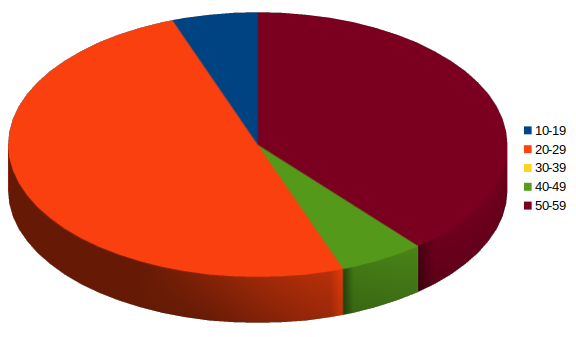
\includegraphics[width=10cm]{images/guiaoR/idades_2.png}
        \caption{Idades da amostragem}
    \end{figure}


O gráfico abaixo mostra a percentagem relativa ao nível de utilização de tecnologias. Como seria de esperar, uma maior parte da amostragem utiliza com frequência tecnologias, e como tal, a probabilidade de utilizar um serviço como o ChatBot seria superior. 
    \begin{figure}[H]
        \centering
        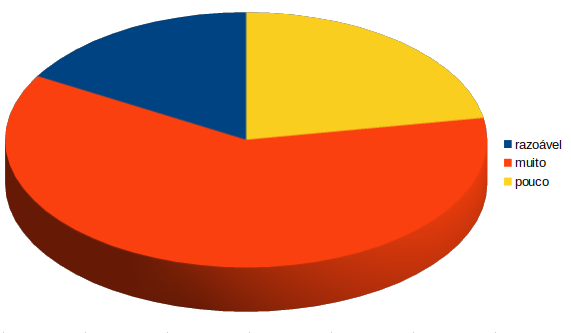
\includegraphics[width=10cm]{images/guiaoR/usoTecnologias_2.png}
        \caption{Nível de utilização de tecnologia da amostragem}
    \end{figure}
    
O gráfico demonstrado em seguida representa o nível de conhecimento na área da tecnologia por parte da amostragem. É possível observar que aproximadamente metade dos testes foram efetuados por pessoas com conhecimento na área. 

    \begin{figure}[H]
        \centering
        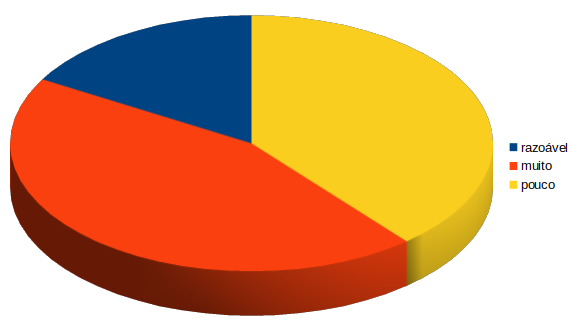
\includegraphics[width=10cm]{images/guiaoR/conhecimento_2.png}
        \caption{Nível de conhecimento na área da tecnologia da amostragem.}
    \end{figure}

\subsection{Metodologia de testes}

Para além das funcionalidades analisadas na primeira avaliação, os testes com o produto final contemplaram ainda o módulo de resolução de problemas e o modo interativo. Desta forma, neste fase de testes foram escolhidas as seguintes funcionalidades:

\begin{itemize}
    \item Cinema Webscraper
        \begin{enumerate}
            \item Cinemas por proximidade.
            \item Cinemas numa determinada localidade.
            \item Próximas sessões num determinado cinema.
            \item Consultar sessões para uma data.
            \item Consultar as próximas estreias.
            \item Consultar os filmes em exibição num cinema.
            \item Consultar detalhes de um filme (utilizando o \textbf{modo interativo}).
            \item Consultar filmes com um determinado critério (utilizando o \textbf{modo interativo}).
            \item Consultar sessões de um filme.
        \end{enumerate}
    \item FS Webscraper
        \begin{enumerate}
            \setcounter{enumi}{9}
            \item Consultar telemóveis em promoção.
            \item Consultar telemóveis dentro de uma gama de preços (utilizando o \textbf{modo interativo}).
            \item Consultar as lojas NOS num dado local.
            \item Consultar as linhas de apoio (utilizando o \textbf{modo interativo}).
            \item Consultar pacotes de um serviço.
        \end{enumerate}
    \item Módulo de resoluções de problemas.
        \begin{enumerate}
        \setcounter{enumi}{14}
            \item Simular a resolução de um problema (``Internet com pouca velocidade'') no serviço de Internet.
            \item Simular a resolução de um problema (``TV avariada'') no serviço TV.
        \end{enumerate}
\end{itemize}

É importante realçar que, dadas as limitações do módulo de resolução de problemas no que diz respeito
à deteção de tipificações a partir de mensagens dos clientes, os testes realizados limitaram consideravelmente
a interação do utilizador com o sistema, sendo o seu intuito apenas o de avaliar o funcionamento deste
módulo no que respeita às soluções propostas.

\subsection{Resultados agregados dos utilizadores}
O \textit{feedback} recolhido nos testes de usabilidade encontra-se agregado, por funcionalidade, na tabela
seguinte:

\begin{longtable}{|c|m{12cm}|}
        \hline
        Pergunta & Sugestões\\ \hline
        1 & \begin{itemize}[leftmargin=0.5cm]
            \setlength\itemsep{0em}
            \item Ter horário de funcionamento dos cinemas.
            \item Acrescentar \emph{link} Google Maps e distância para cada cinema.
        \end{itemize}\\ \hline
        2 & \begin{itemize}[leftmargin=0.5cm]
            \setlength\itemsep{0em}
            \item Ao apresentar um cinema dizer quais os filmes que tem em exibição.
            \item Melhorar frases e forma de apresentação.
            \item Melhorar detecção de localidades.
        \end{itemize} \\ \hline
        3 & \begin{itemize}[leftmargin=0.5cm]
            \setlength\itemsep{0em}
            \item Acrescentar a duração dos filmes.
        \end{itemize}\\ \hline
        4 & \begin{itemize}[leftmargin=0.5cm]
            \setlength\itemsep{0em}
            \item Tornar mais claros os pedidos de informação aos utilizadores.
            \item Detetar os dias de segunda a domingo.
            \item Ter a imagem do filmes nas sessões.
        \end{itemize}\\ \hline
        5 & \begin{itemize}[leftmargin=0.5cm]
            \setlength\itemsep{0em}
            \item Referir a data de estreia dos filmes.
        \end{itemize}\\ \hline
        6 & \begin{itemize}[leftmargin=0.5cm]
            \setlength\itemsep{0em}
            \item Devolver mais informações dos filmes.
            \item Links para mais informações de cada filme.
        \end{itemize}\\ \hline
        7 & \begin{itemize}[leftmargin=0.5cm]
            \setlength\itemsep{0em}
            \item Melhorar a forma como são escritas algumas opções.
        \end{itemize}\\ \hline
        8 & \begin{itemize}[leftmargin=0.5cm]
            \setlength\itemsep{0em}
            \item No primeiro menu mudar a opção de ``cinemas'' ou ``sessões''.
            \item Na filtragem de filmes mudar a opção de ``cast'' para ``elenco''.
            \item Mudar a opção ``filmes específicos'' que não é clara.
            \item Melhorar pedido de faixa etária.
        \end{itemize}\\ \hline
        9 & \begin{itemize}[leftmargin=0.5cm]
            \setlength\itemsep{0em}
            \item Melhorar a detecção de filmes nas frases dos utilizadores.
            \item Manter um contexto entre perguntas da mesma categoria consecutivas.
        \end{itemize}\\ \hline
        10 & \begin{itemize}[leftmargin=0.5cm]
            \setlength\itemsep{0em}
            \item Melhorar a detecção de frases.
            \item Apresentar também aqui o processador, a RAM e a câmara.
            \item Tornar a apresentação dos links mais concisas.
            \item Tornar a escolha de filtros mais intuitiva.
        \end{itemize}\\ \hline
        11 & \begin{itemize}[leftmargin=0.5cm]
            \setlength\itemsep{0em}
            \item Destacar a opção de apresentar resultados.
            \item Apresentar os telemóveis ordenados por preços.
        \end{itemize}\\ \hline
        12 & \begin{itemize}[leftmargin=0.5cm]
            \setlength\itemsep{0em}
            \item Melhorar a forma de pesquisa das lojas (exemplo: Braga devolveu também uma loja de Bragança).
            \item Acrescentar link Google Maps para cada loja.
        \end{itemize}\\ \hline
        13 & \begin{itemize}[leftmargin=0.5cm]
            \setlength\itemsep{0em}
            \item Ter uma descrição de cada linha de apoio (informação que temos em posse mas não é apresentada).
        \end{itemize}\\ \hline
        14 & \begin{itemize}[leftmargin=0.5cm]
            \setlength\itemsep{0em}
            \item Melhorar detecção de frases.
            \item Apresentar \emph{link} para obter mais informações.
        \end{itemize}\\ \hline
        15, 16 & \begin{itemize}[leftmargin=0.5cm]
            \setlength\itemsep{0em}
            \item Melhorar a detecção do problema do cliente.
            \item Na autenticação, perguntar pelo telemóvel e NIF em mensagens separadas.
        \end{itemize}\\ \hline
        Geral & \begin{itemize}[leftmargin=0.5cm]
            \setlength\itemsep{0em}
            \item Não sair logo do modo interativo quando se termina a obtenção de alguma informação.
        \end{itemize}\\ \hline
    \caption{Sugestões dos utilizadores nos testes com o produto final.}
    \label{tab:my_label2}
\end{longtable}

\subsection{Conclusões}

A análise do \textit{feedback} recolhido permite observar que diversas sugestões feitas pelos utilizadores
dizem respeito a itens previamente referidos e que não foram implementados, quer pela indisponibilidade da
informação ou pela prioridade atribuída aos mesmos. Por outro lado, estes testes permitem ainda concluir
que a maior limitação do sistema prende-se com a sua capacidade de interpretação de linguagem natural e de
lidar com a variabilidade inerente ao discurso coloquial. Esta observação reforça a utilidade de um modo
interativo que serve de \textit{fallback} para situações em que o sistema não seja capaz de categorizar
as perguntas dos utilizadores corretamente.

\newpage
\begin{appendices}

\section{Teste protótipo}

\subsection{Objetivos}
\begin{enumerate}
    \item Testar capacidade de resposta (funcionalidades) do microserviço Cinemas
    \item Testar capacidade de resposta (funcionalidades) do microserviço FS 
    \item Testar qualidade das respostas às perguntas do utilizador
    \item Averiguar a variabilidade de \textit{inputs} para cada use case
\end{enumerate}

\subsection{Guião}
\begin{enumerate}
    \item Pedir ao utilizador para consultar os cinemas mais próximos.
    \item Pedir para consultar os cinemas que existem em Lisboa.
    \begin{figure}[H]
        \centering
        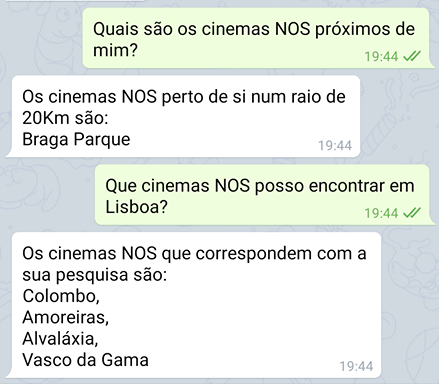
\includegraphics[width=5cm]{images/guiaoP/2.png}
    \end{figure}
    \item Pedir ao utilizador para consultar os filmes num determinado cinema (ou por search\_term). Neste caso, com o search\_term Algarve.
    \begin{figure}[H]
        \centering
        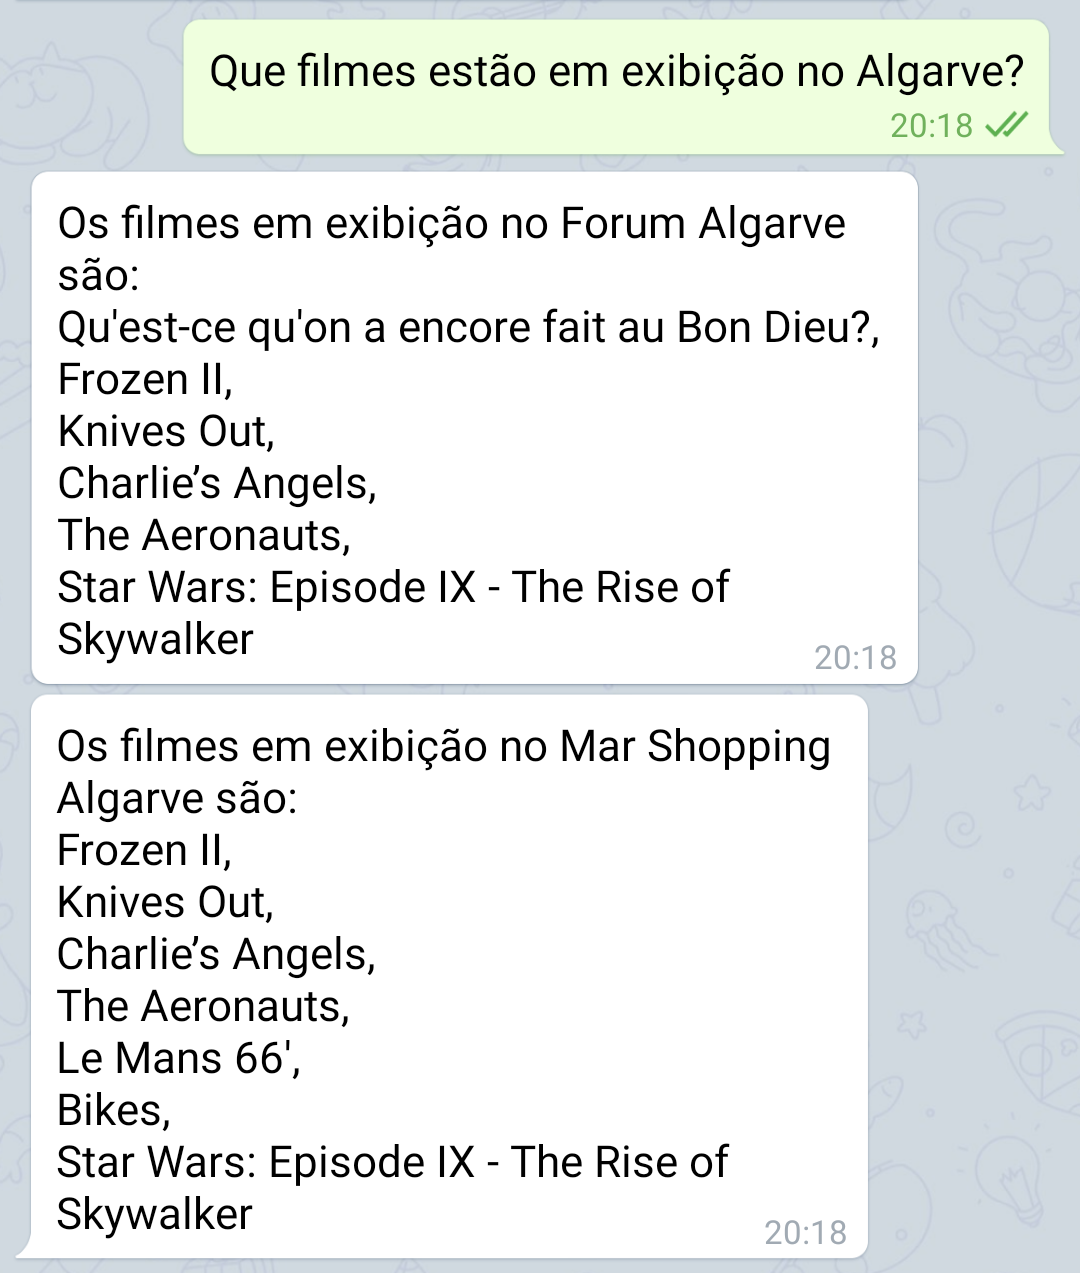
\includegraphics[width=5cm]{images/guiaoP/3.png}
    \end{figure}
    \item Procurar filmes por determinado critério (elenco, sinopse, género). Neste caso, filmes em que entra o Kevin Hart.
    \begin{figure}[H]
        \centering
        \subfloat{{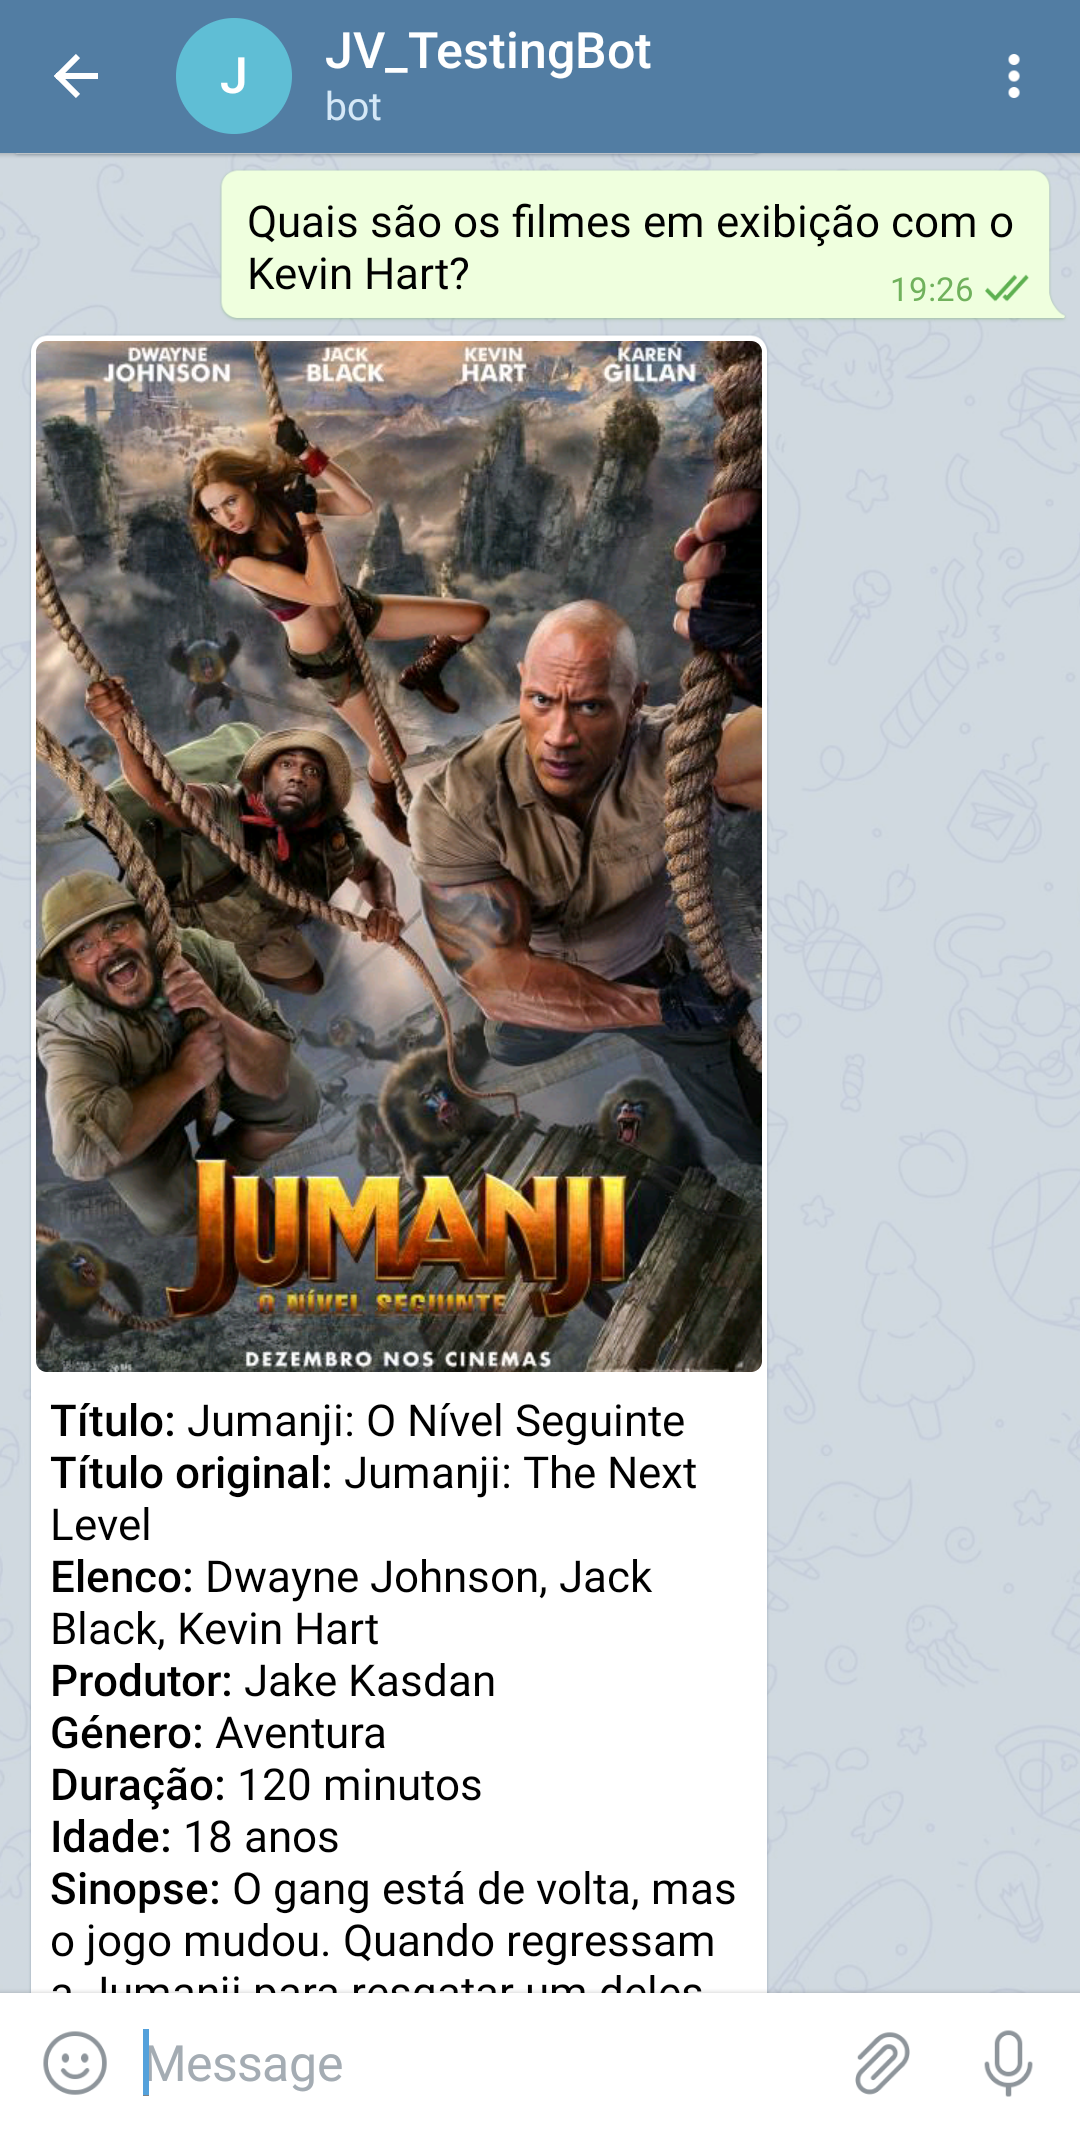
\includegraphics[width=4cm]{images/guiaoP/4_1.png}}}
        \qquad
        \subfloat{{
\includegraphics[width=4cm]{images/guiaoP/4_2.png}}}
    \end{figure}
    \item Pedir ao utilizador para consultar as próximas estreias.
    \begin{figure}[H]
        \centering
        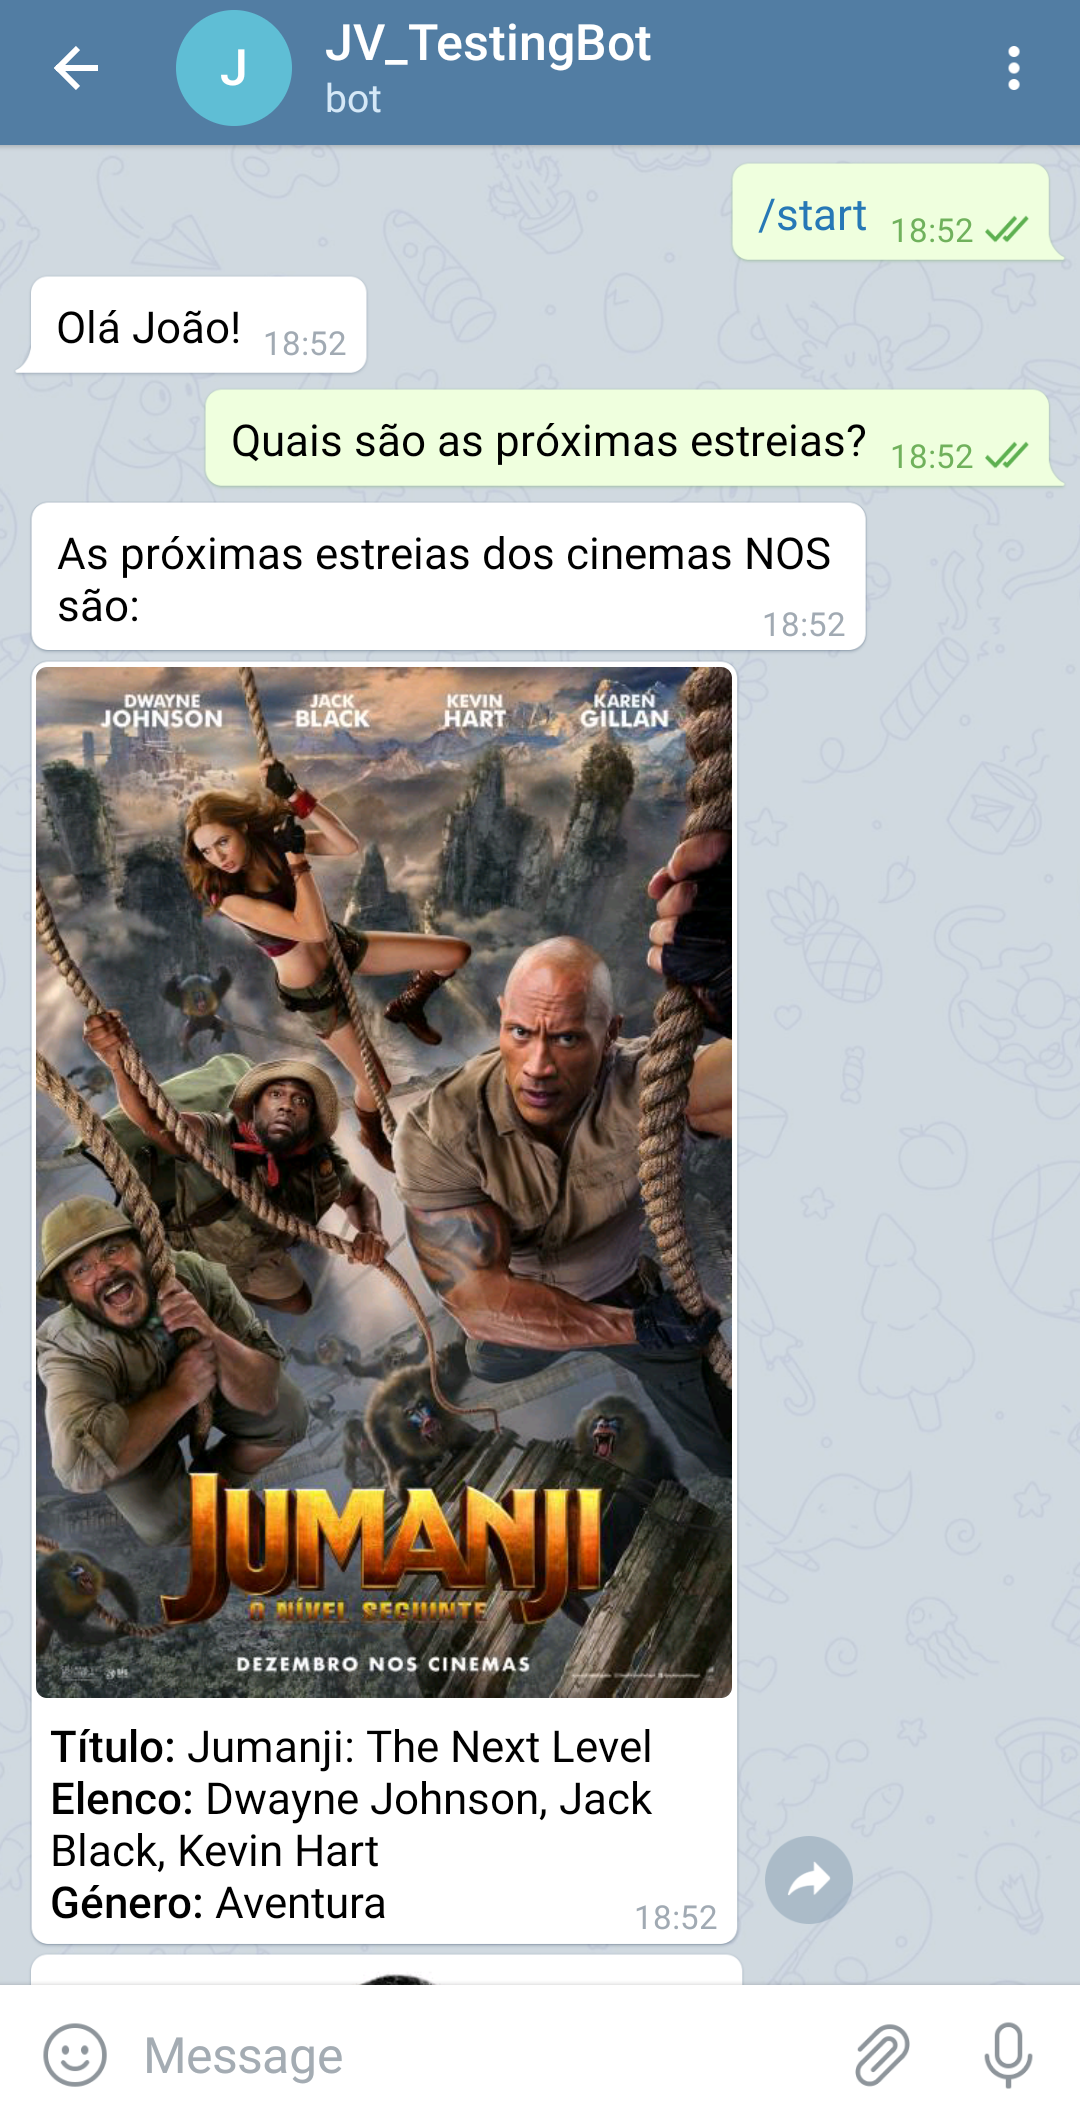
\includegraphics[width=4cm]{images/guiaoP/5.png}
    \end{figure}
    \item Pedir ao utilizador para consultar as próximas sessões num determinado cinema (Braga Parque por ser o mais perto).
    \begin{figure}[H]
        \centering
        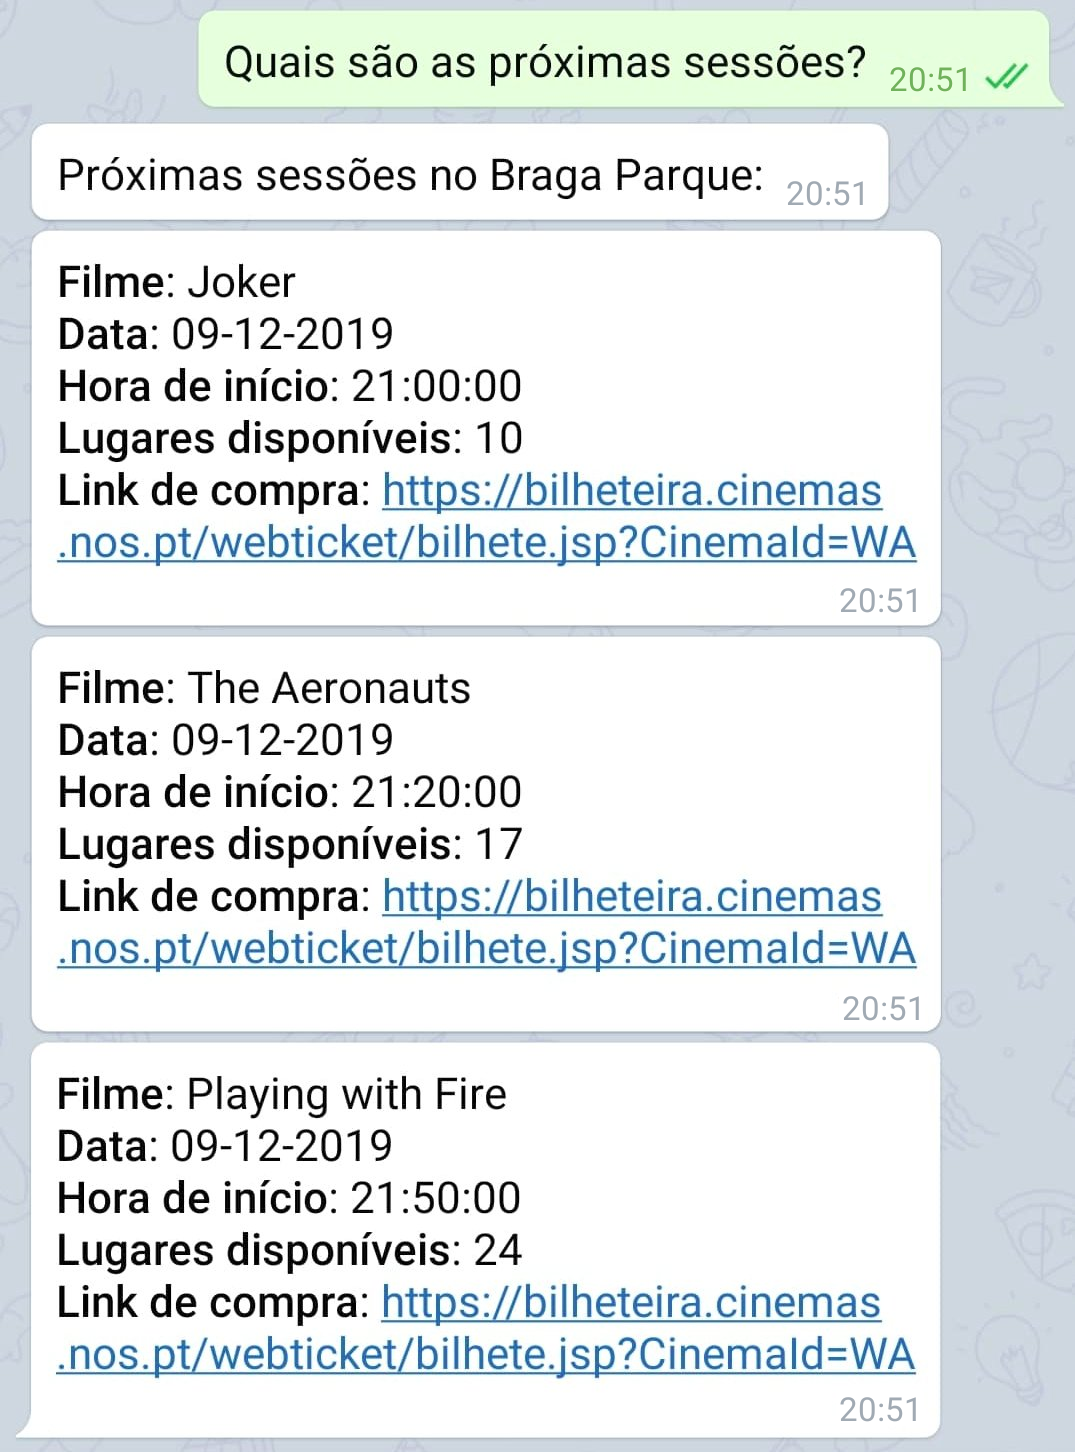
\includegraphics[width=5cm]{images/guiaoP/6.png}
    \end{figure}
    \item Pedir ao utilizador para consultar sessões para um determinado filme (\textit{Countdown}).
    \begin{figure}[H]
        \centering
        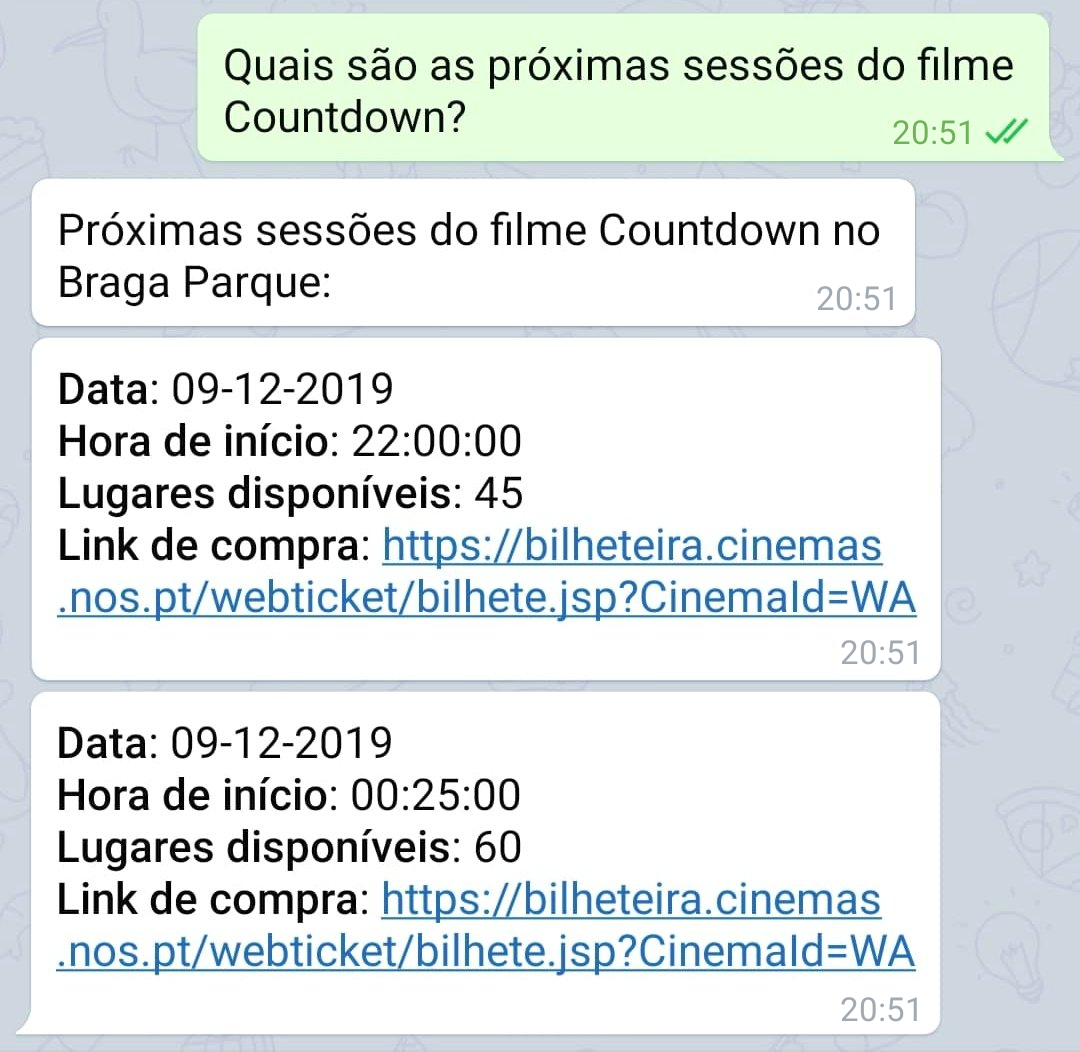
\includegraphics[width=5cm]{images/guiaoP/7.png}
    \end{figure}
    \item Pedir ao utilizador para consultar a linha de apoio para esclarecimentos sobre pacotes da NOS.
    \begin{figure}[H]
        \centering
        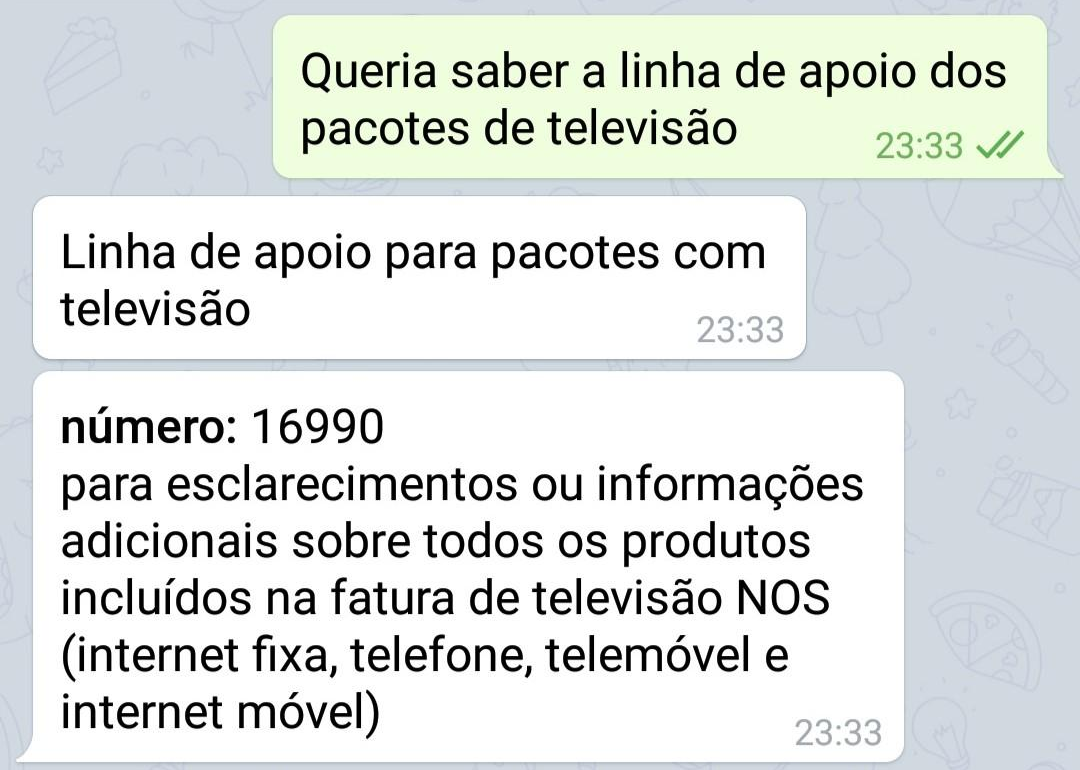
\includegraphics[width=5cm]{images/guiaoP/8.png}
    \end{figure}
    \item Pedir ao utilizador para consultar as informações de um modelo de telemóvel.
    \begin{figure}[H]
        \centering
        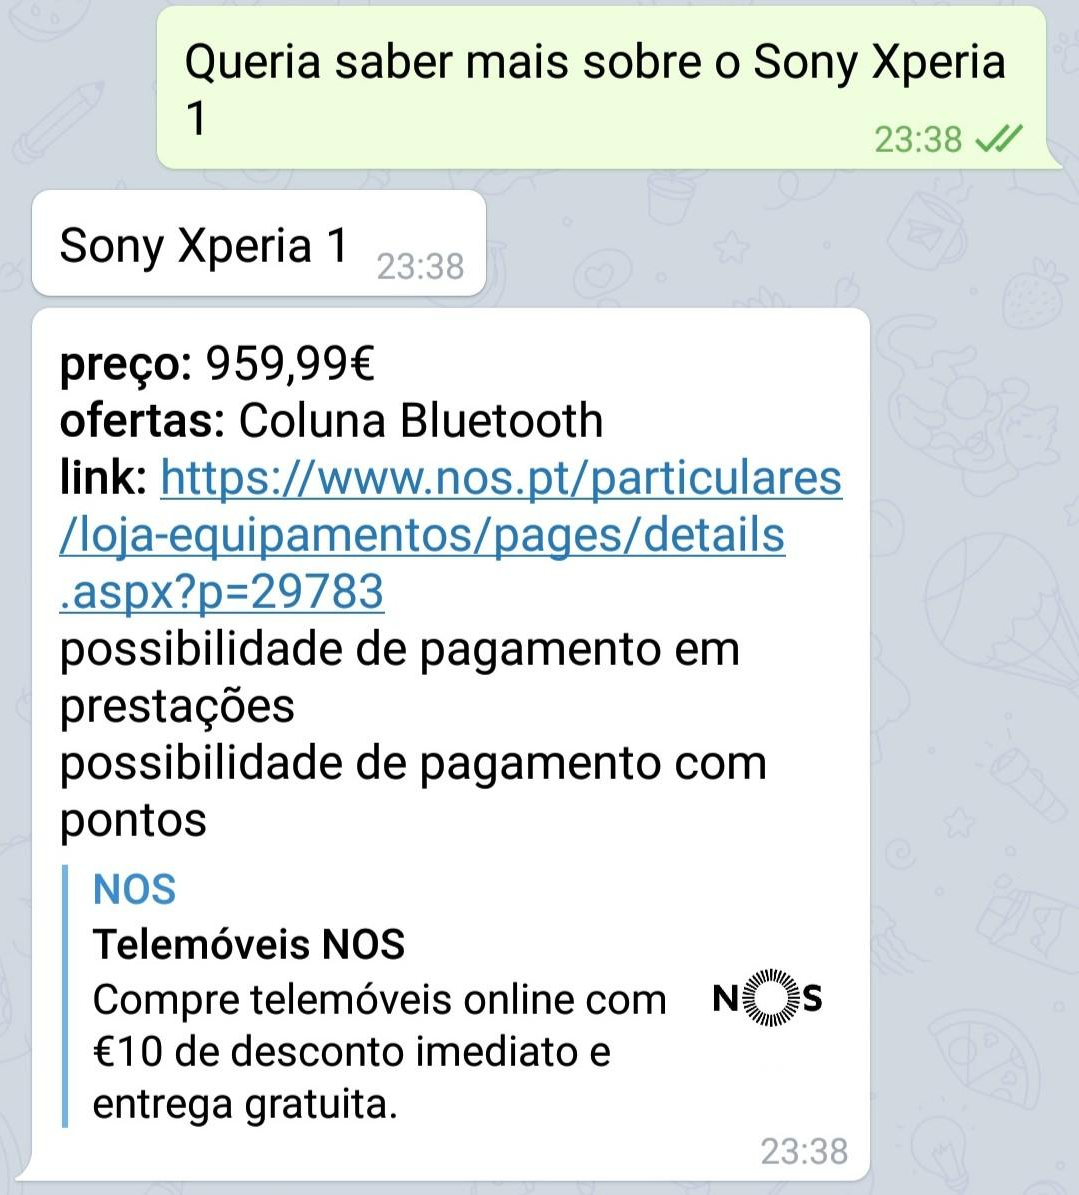
\includegraphics[width=5cm]{images/guiaoP/9.png}
    \end{figure}
    \item Pedir ao utilizador para consultar todos os telemóveis em promoção.
    \begin{figure}[H]
        \centering
        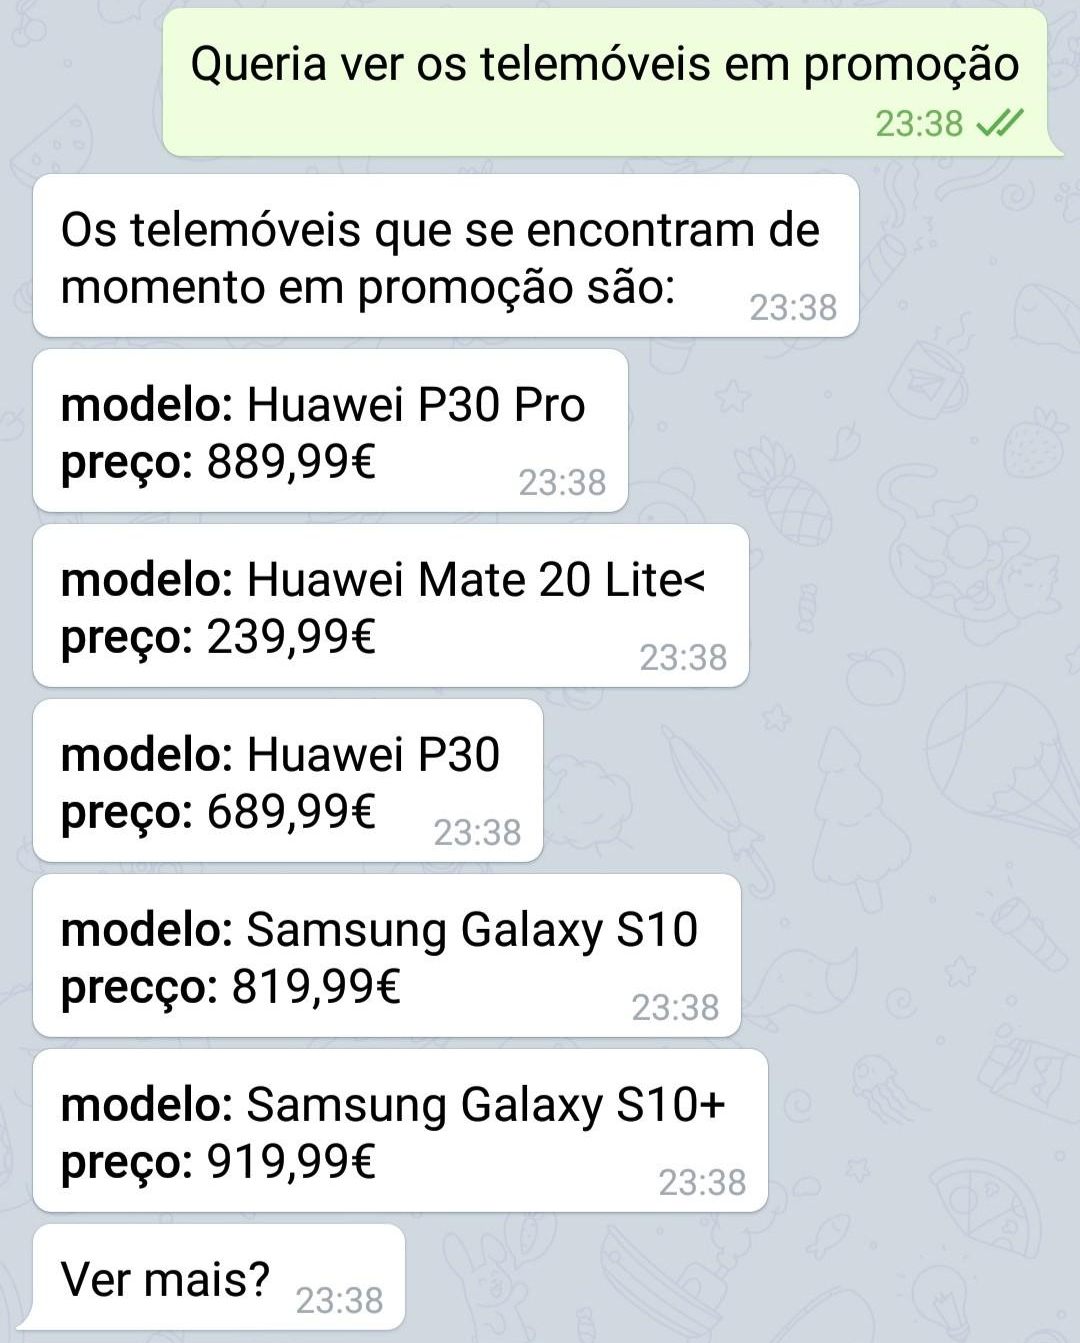
\includegraphics[width=5cm]{images/guiaoP/10.png}
    \end{figure}
    \item Pedir ao utilizador para consultar tarifários WTF.
    \begin{figure}[H]
        \centering
        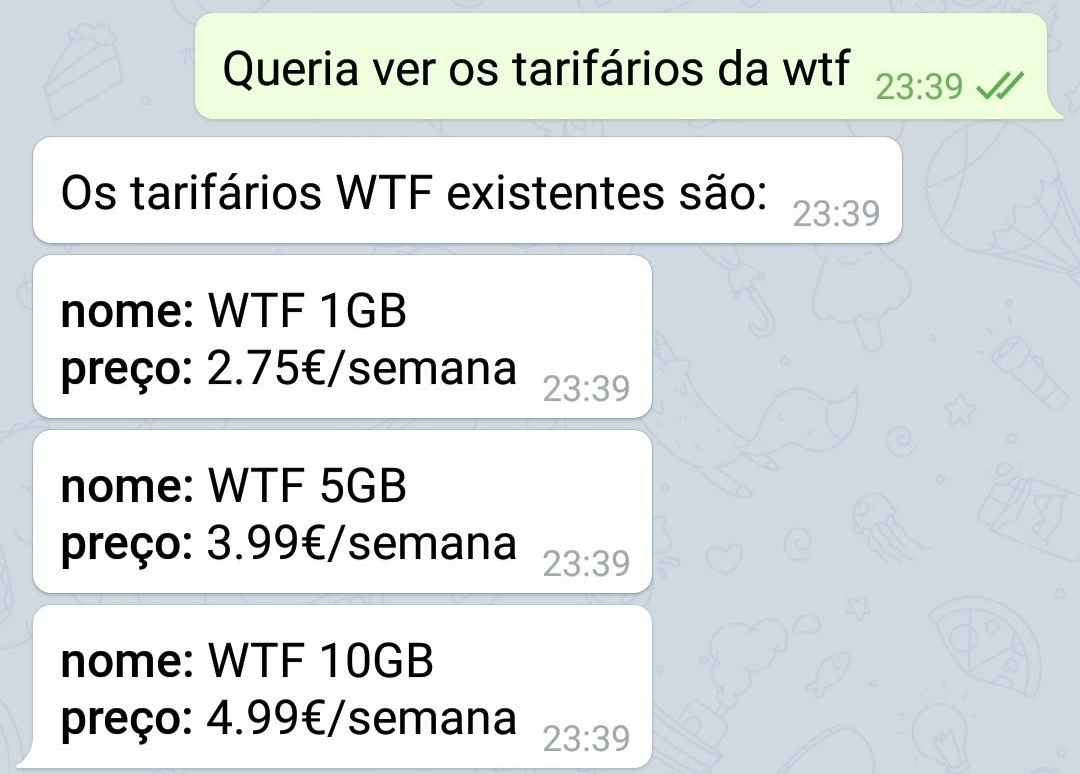
\includegraphics[width=5cm]{images/guiaoP/11.png}
    \end{figure}
    \item Pedir ao utilizador para consultar os pacotes fibra numa gama de valores.
    \begin{figure}[H]
        \centering
        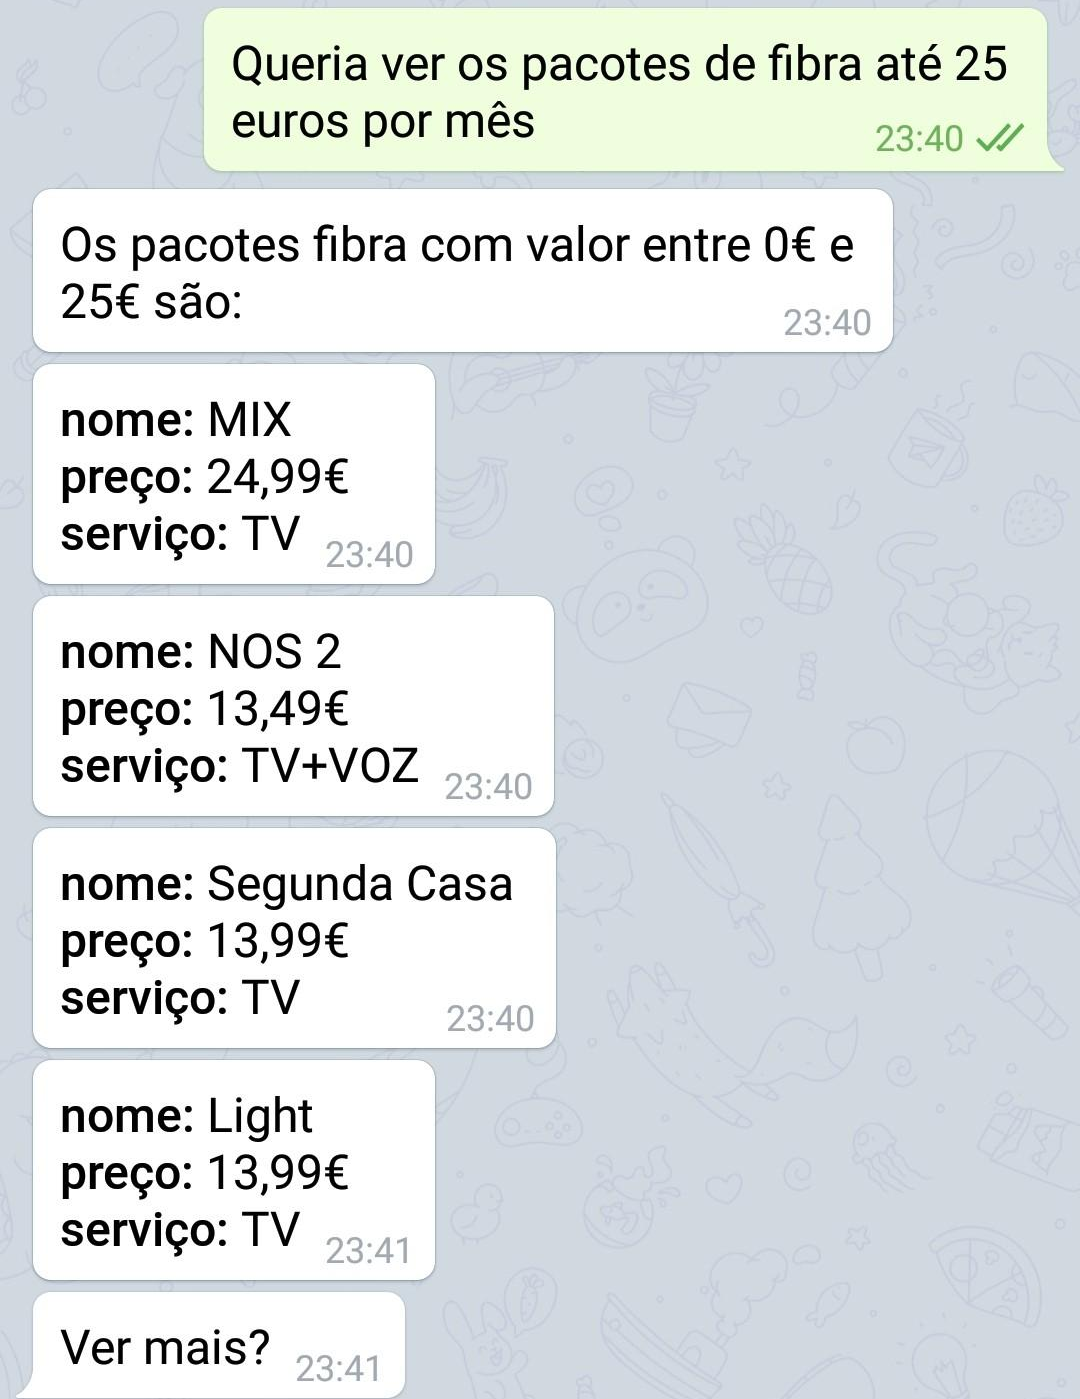
\includegraphics[width=5cm]{images/guiaoP/12.png}
    \end{figure}
    \item Pedir ao utilizador para consultar os pacotes satélite com determinado serviço.
    \begin{figure}[H]
        \centering
        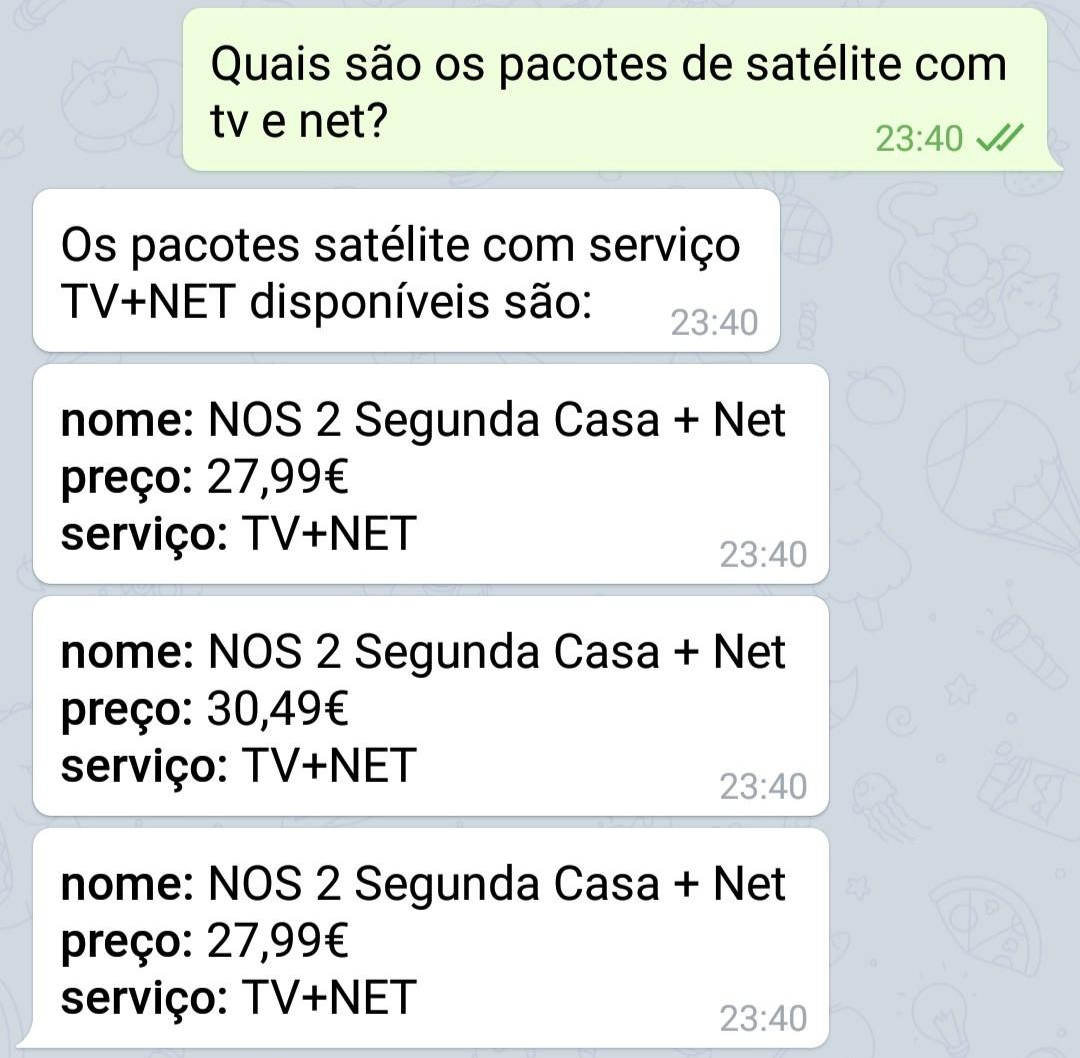
\includegraphics[width=5cm]{images/guiaoP/13.png}
    \end{figure}
    \item Pedir ao utilizador para consultar lojas NOS numa determinada cidade.
    \begin{figure}[H]
        \centering
        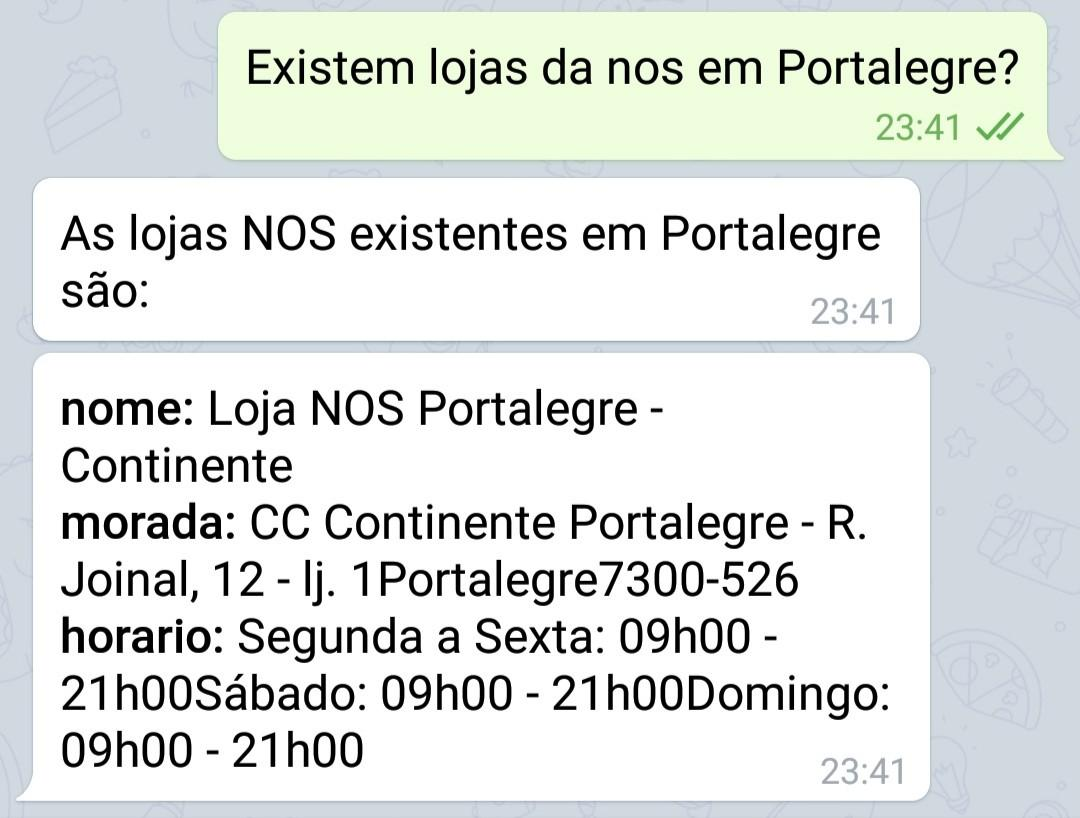
\includegraphics[width=5cm]{images/guiaoP/14.png}
    \end{figure}
\end{enumerate}

\newpage
\section{Guião do teste com o Produto Final}
\begin{enumerate}
    \item Consultar os cinemas mais próximos de si.
    \begin{figure}[H]
        \centering
        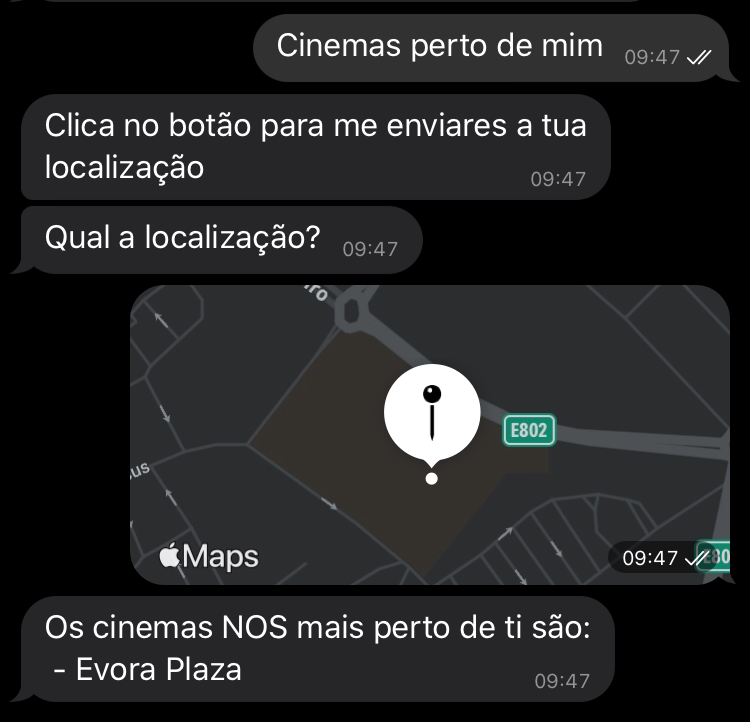
\includegraphics[width=5cm]{images/guiaoR/1.png}
    \end{figure}
    \item Consultar os cinemas que existem em <local> (e.g. Bucelas).
    \begin{figure}[H]
        \centering
        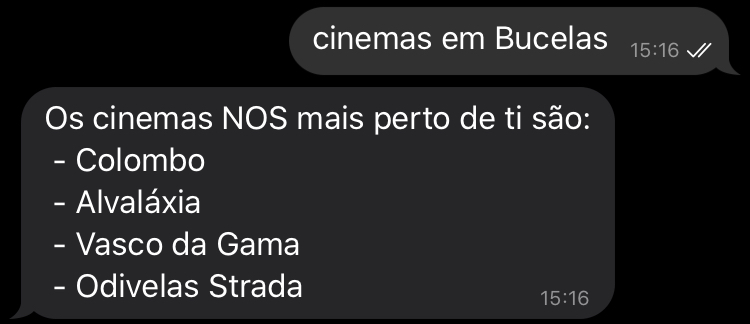
\includegraphics[width=5cm]{images/guiaoR/2.jpg}
    \end{figure}
    \item Consultar as próximas sessões num determinado cinema (e.g. Braga).
    \begin{figure}[H]
        \centering
        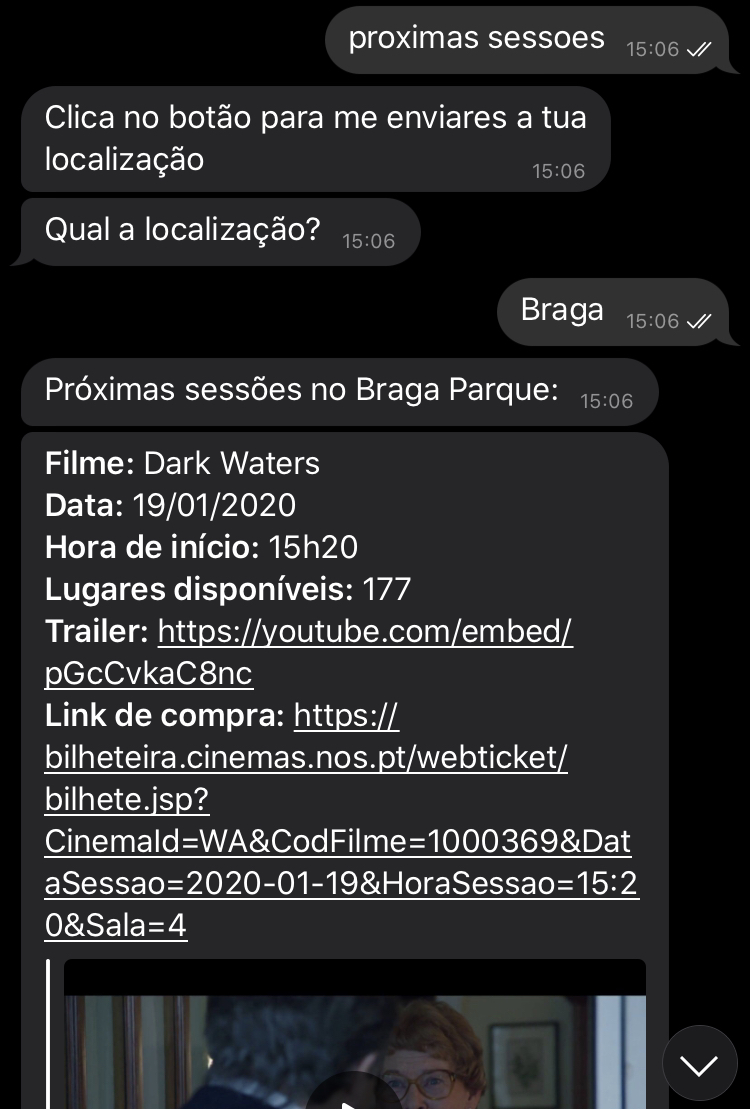
\includegraphics[width=5cm]{images/guiaoR/3.jpg}
    \end{figure}
    \item Consultar sessões para um determinado dia, nesse cinema (e.g. Évora).
    \begin{figure}[H]
        \centering
        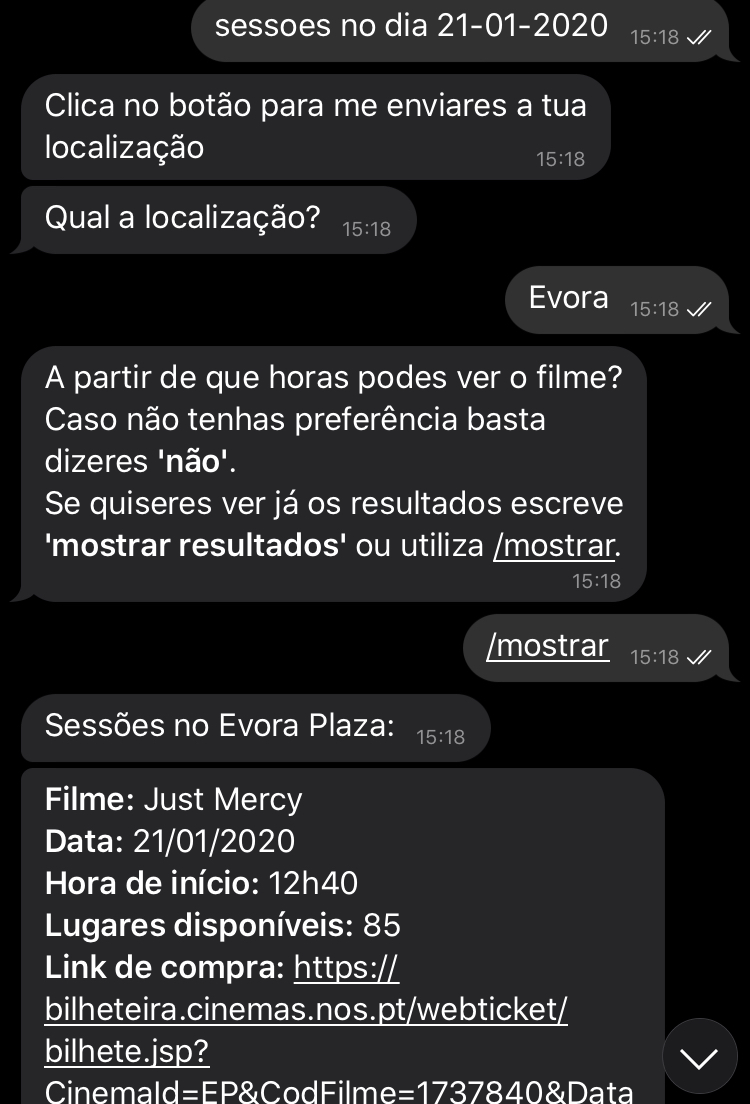
\includegraphics[width=5cm]{images/guiaoR/4.jpg}
    \end{figure}
    \item Consultar próximas estreias.
    \begin{figure}[H]
        \centering
        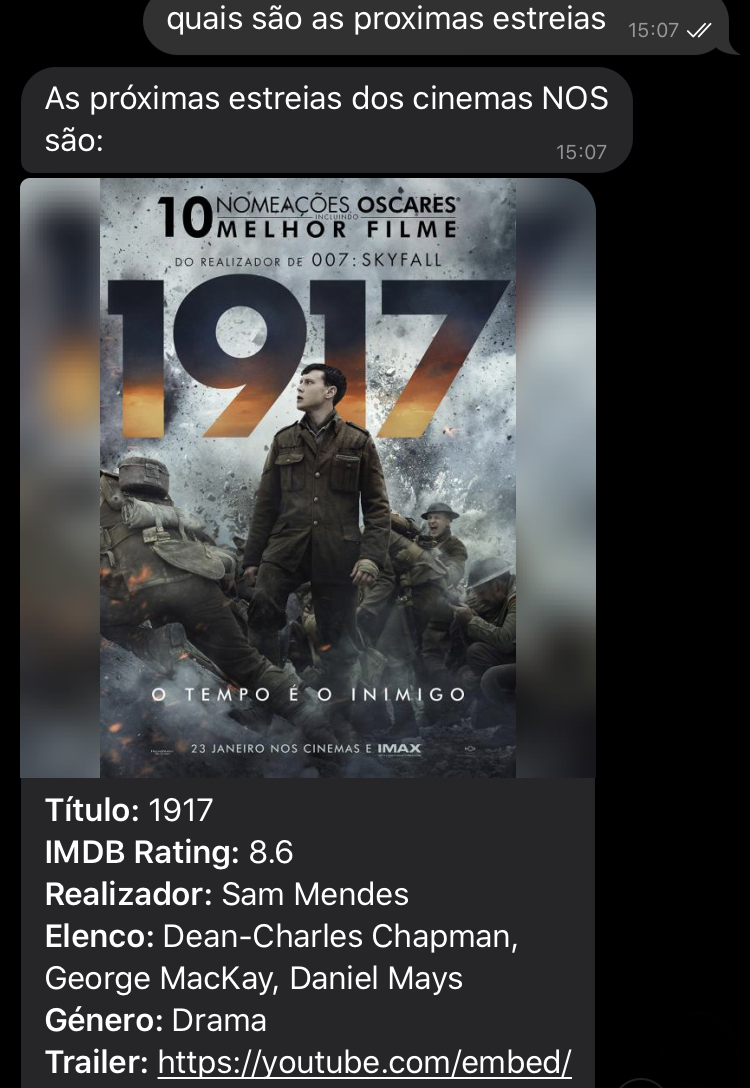
\includegraphics[width=4cm]{images/guiaoR/5.jpg}
    \end{figure}
    \item Consultar os filmes num determinado cinema (e.g. Braga).
    \begin{figure}[H]
        \centering
        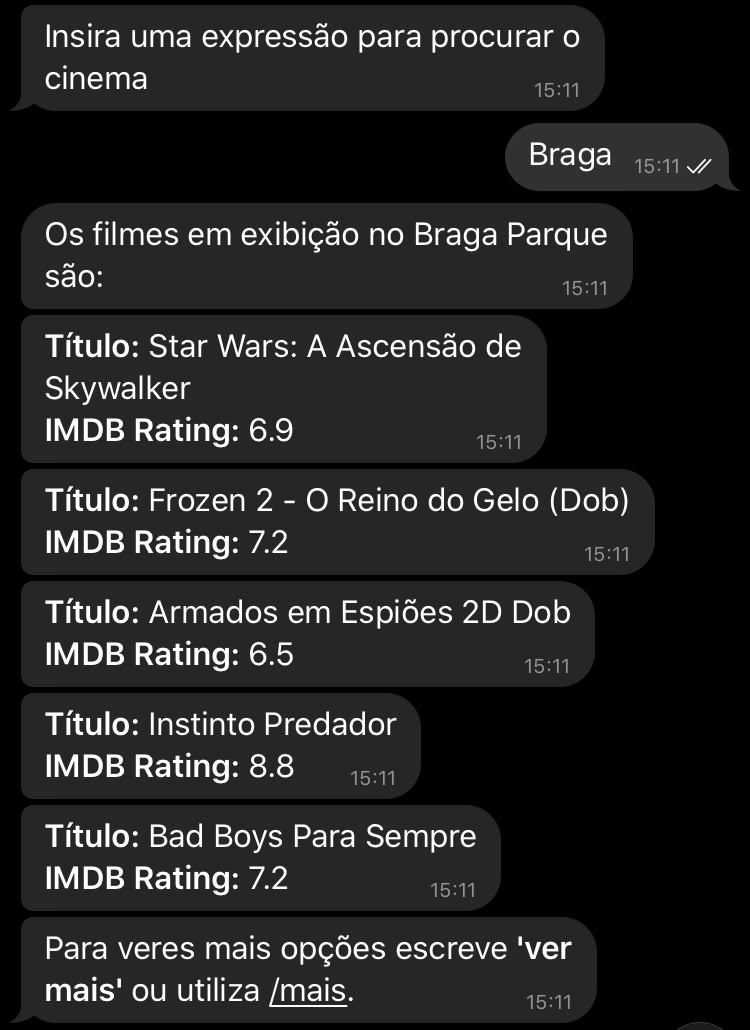
\includegraphics[width=5cm]{images/guiaoR/6.jpg}
    \end{figure}
    \item Consultar detalhes de um determinado filme (modo interativo) (e.g. Instinto Predador)
    \begin{figure}[H]
        \centering
        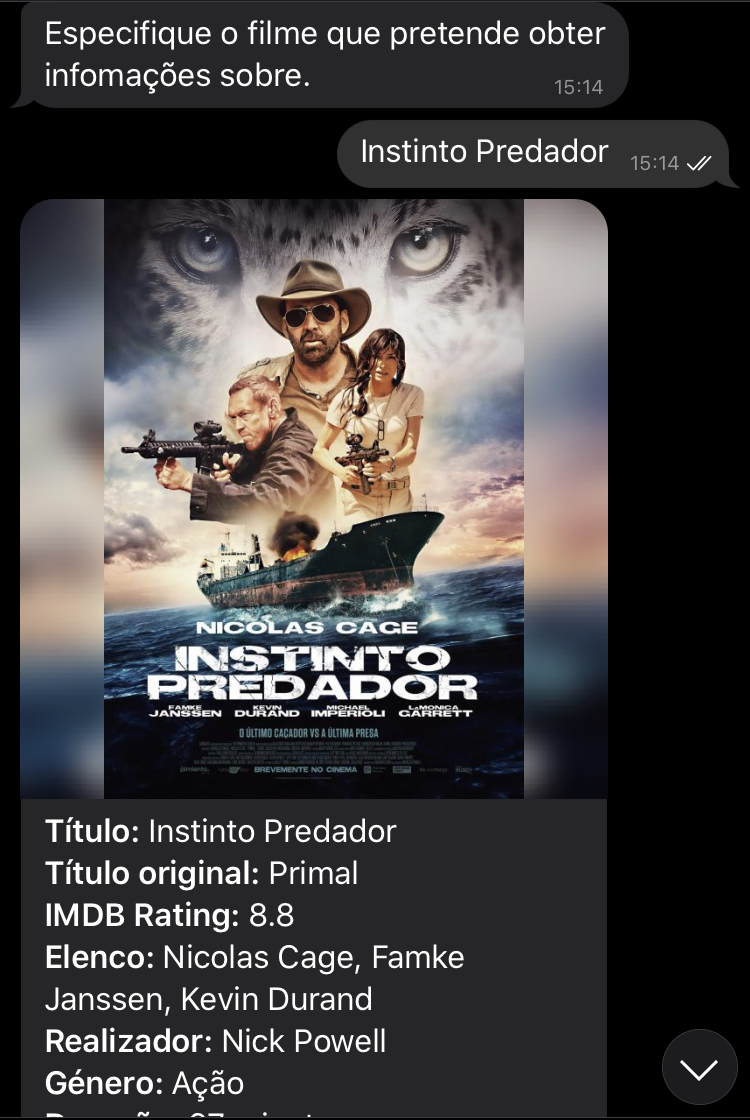
\includegraphics[width=5cm]{images/guiaoR/7.jpg}
    \end{figure}
    \item Consultar filmes de acordo com um determinado parâmetro/critério (modo interativo) (e.g. Elenco com Rosamund Pike).
    \begin{figure}[H]
        \centering
        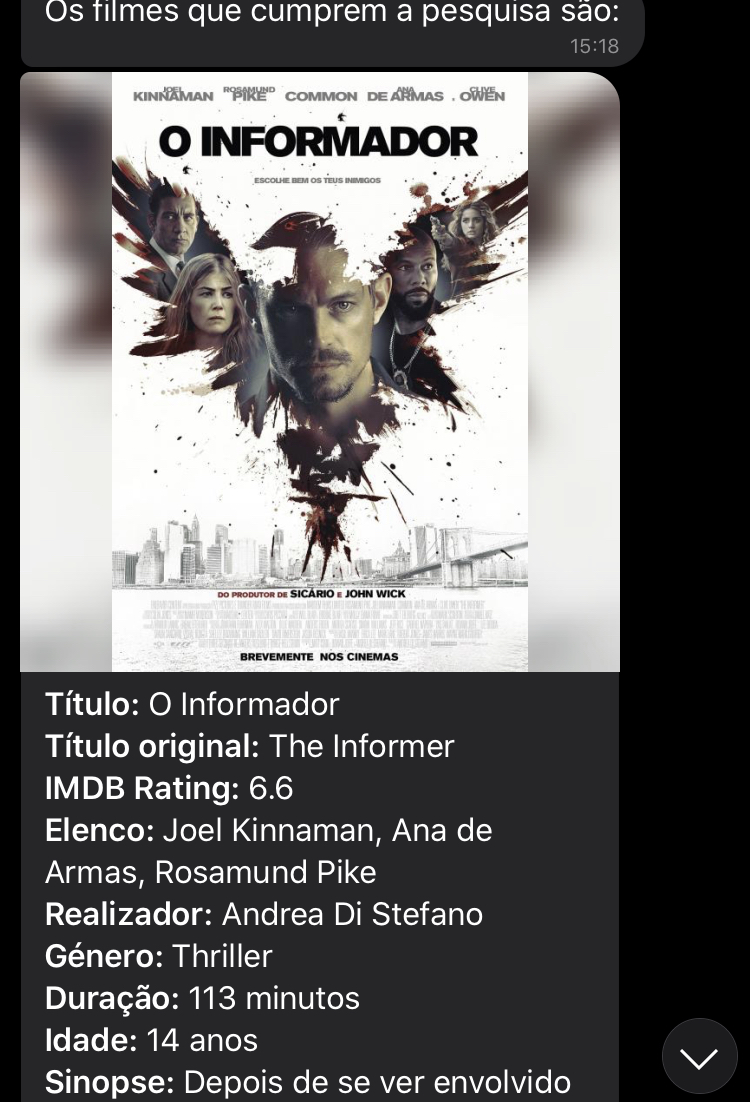
\includegraphics[width=5cm]{images/guiaoR/8.jpg}
    \end{figure}
    \item Consultar sessões de um determinado filme (e.g. The Informer em Évora)
    \begin{figure}[H]
        \centering
        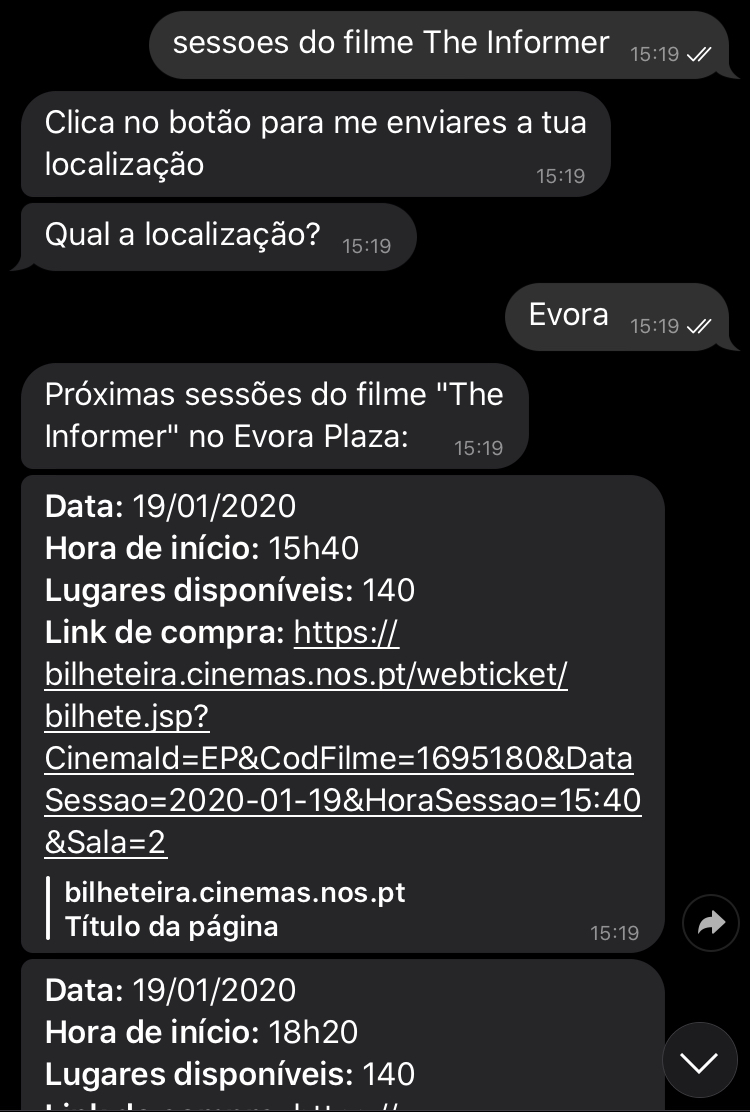
\includegraphics[width=5cm]{images/guiaoR/9.jpg}
    \end{figure}
    \item Consultar todos os telemóveis em promoção.
    \begin{figure}[H]
        \centering
        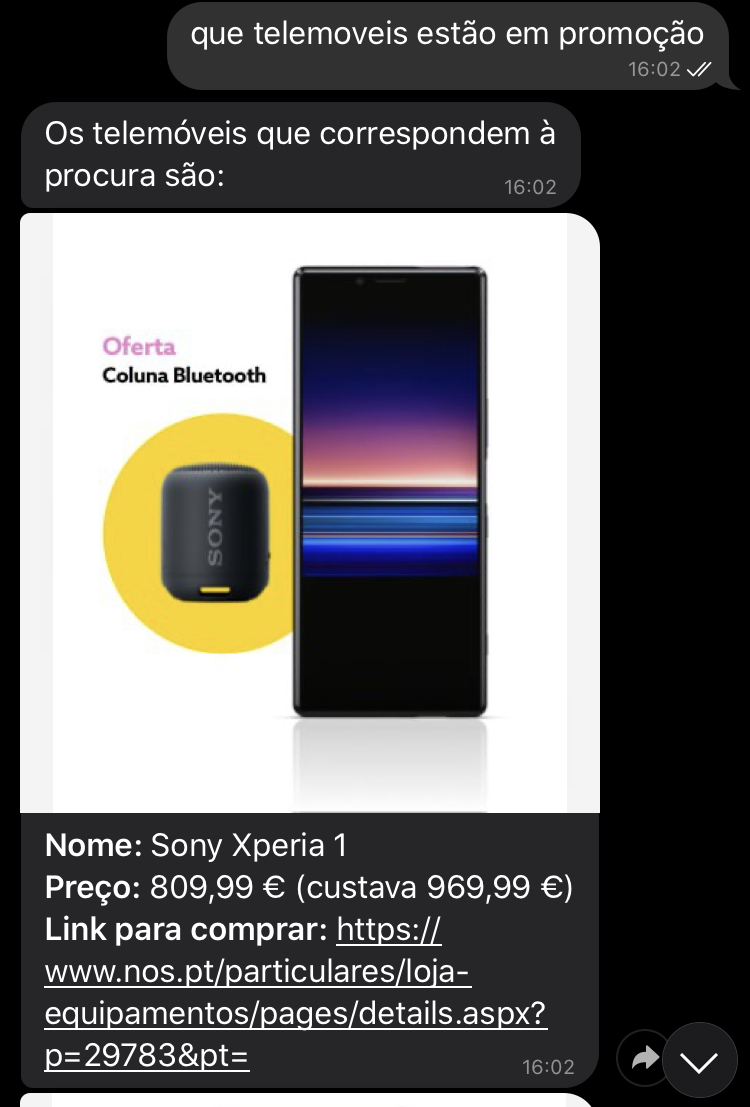
\includegraphics[width=5cm]{images/guiaoR/10.jpg}
    \end{figure}
    \item Consultar telemóveis até determinado preço (modo interativo).
    \item Consultar lojas NOS num determinado local (e.g. Porto).
    \begin{figure}[H]
        \centering
        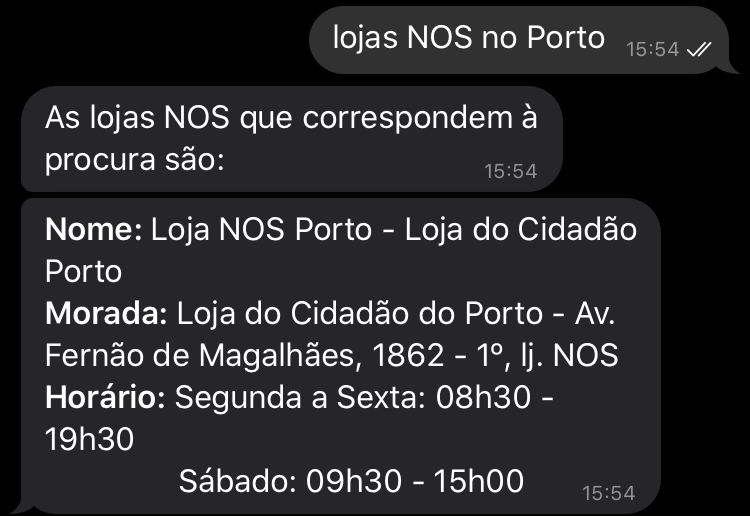
\includegraphics[width=5cm]{images/guiaoR/12.jpg}
    \end{figure}
    \item Consultar as linhas de apoio (modo interativo).
    \begin{figure}[H]
        \centering
        \subfloat{{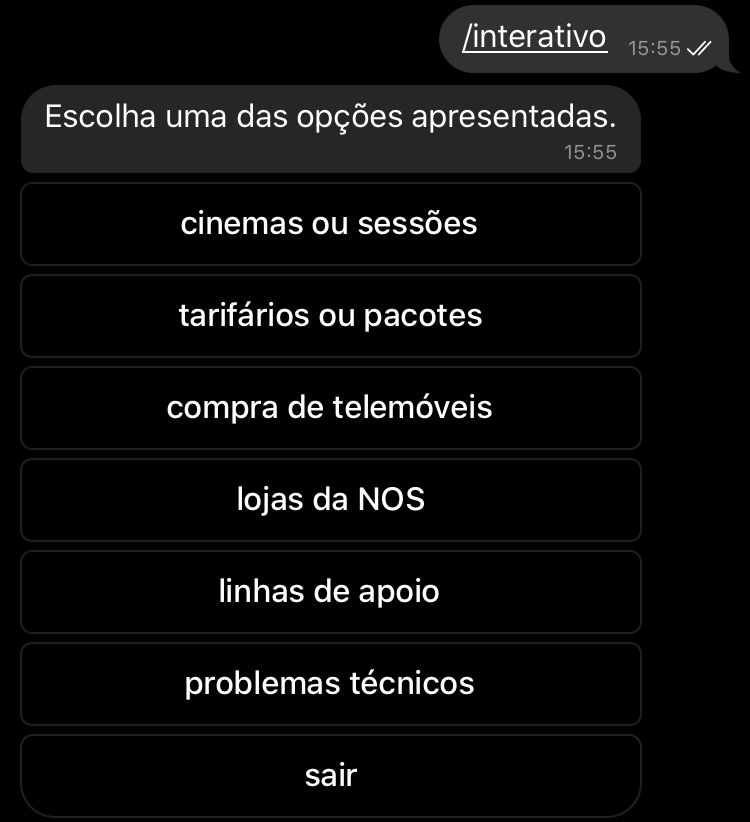
\includegraphics[width=5cm]{images/guiaoR/13_1.png}}}
        \qquad
        \subfloat{{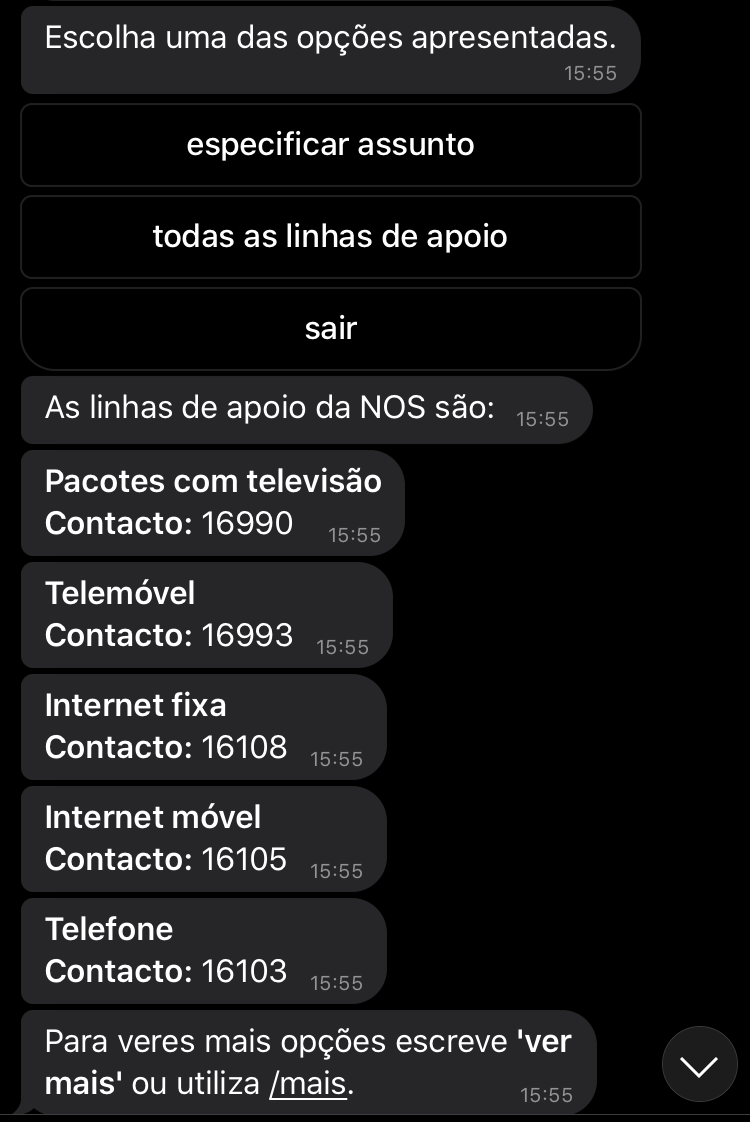
\includegraphics[width=4cm]{images/guiaoR/13_2.png}}}
    \end{figure}
    \item Consultar pacotes de um serviço (e.g. TV).
    \begin{figure}[H]
        \centering
        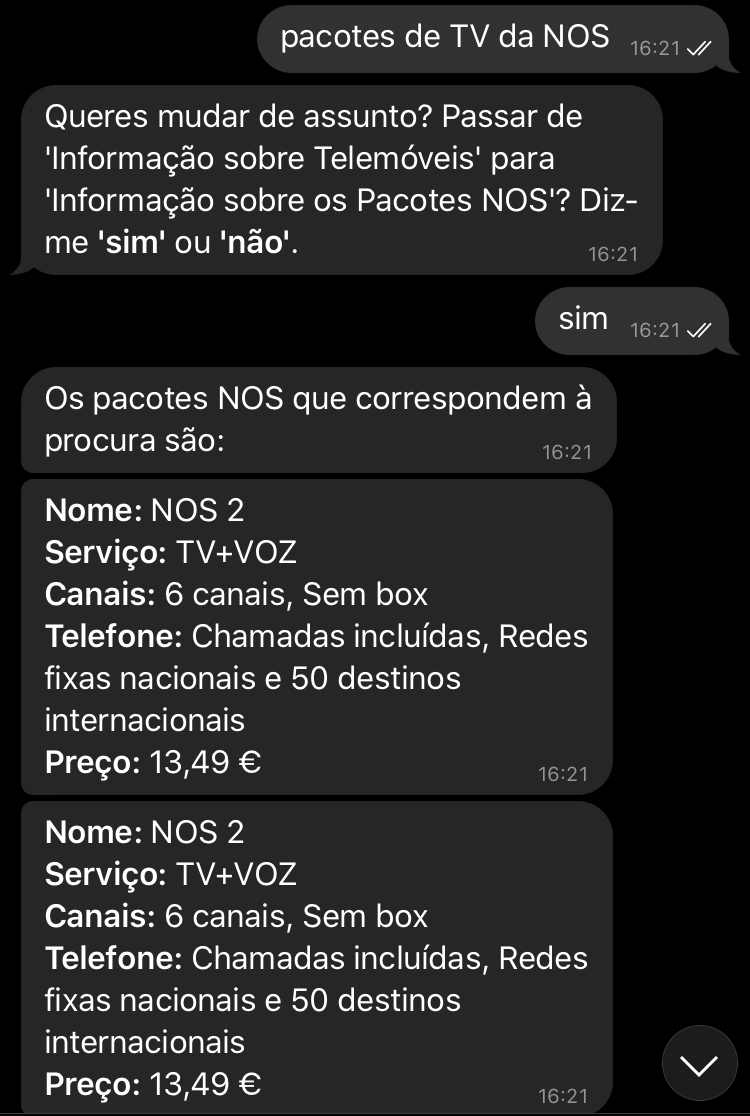
\includegraphics[width=5cm]{images/guiaoR/14.jpg}
    \end{figure}
    \item Simular resolução de problema.
    \begin{itemize}
        \item Dados de autenticação: 968888888 111111111
        \item Serviço: Internet
        \item Problema: Internet com pouca velocidade
        \item Responder não à primeira solução, aceitar a segunda
    \end{itemize}
    \begin{figure}[H]
        \centering
        \subfloat{{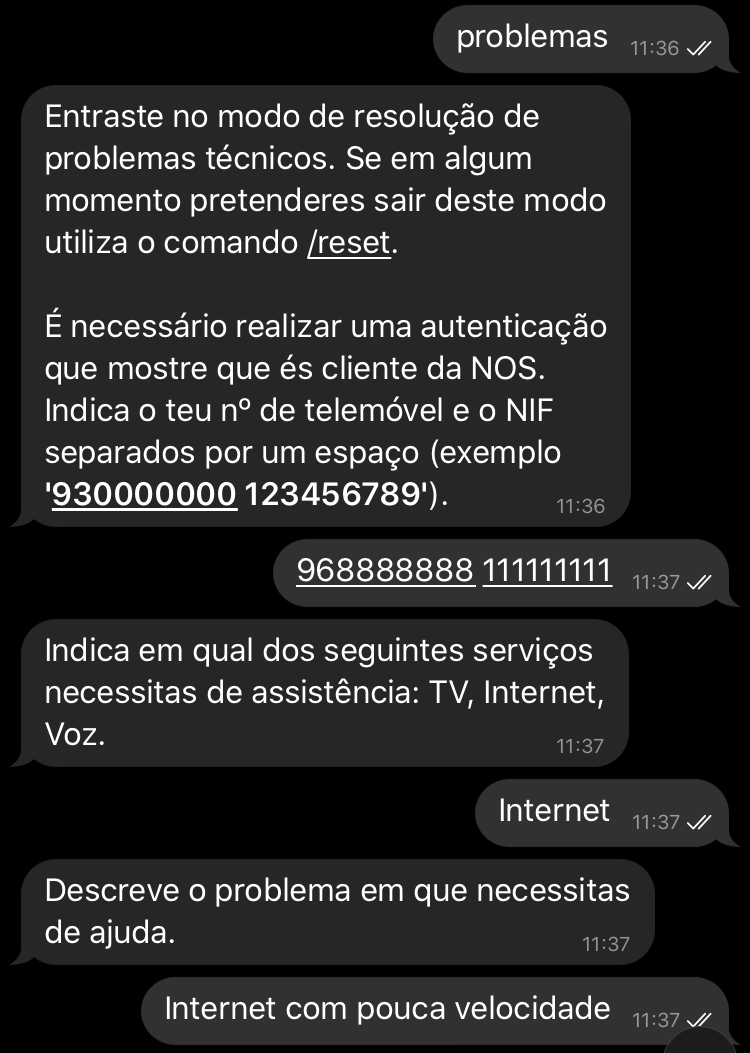
\includegraphics[width=4cm]{images/guiaoR/15_1.png}}}
        \qquad
        \subfloat{{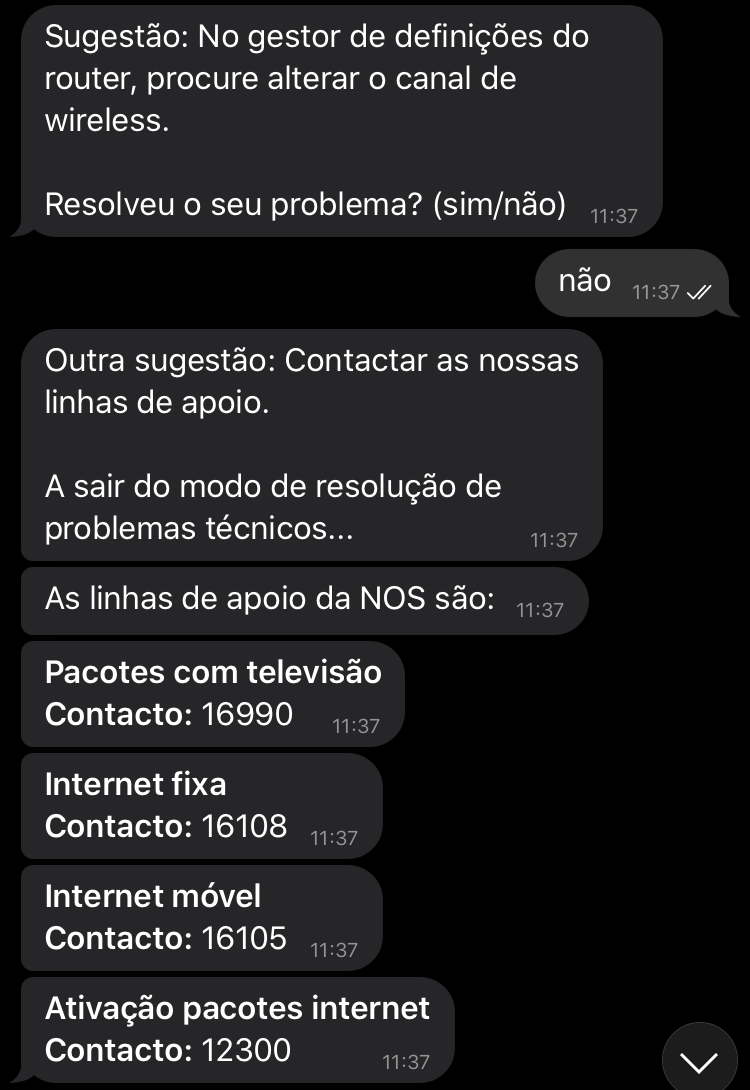
\includegraphics[width=4cm]{images/guiaoR/15_2.png}}}
    \end{figure}
    \item Simular resolução de problema.
    \begin{itemize}
        \item Dados de autenticação: 933333333 111111111
        \item Serviço: TV
        \item Problema: TV avariada
        \item Aceitar a primeira solução
    \end{itemize}
    \begin{figure}[H]
        \centering
        \subfloat{{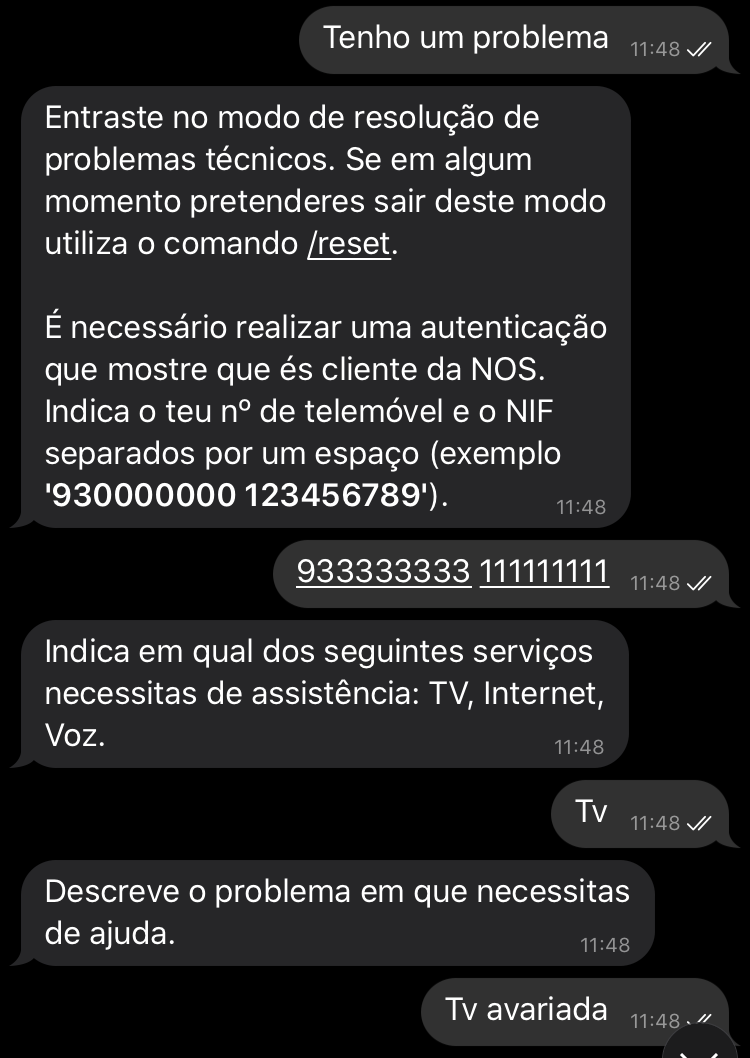
\includegraphics[width=4cm]{images/guiaoR/16_1.png}}}
        \qquad
        \subfloat{{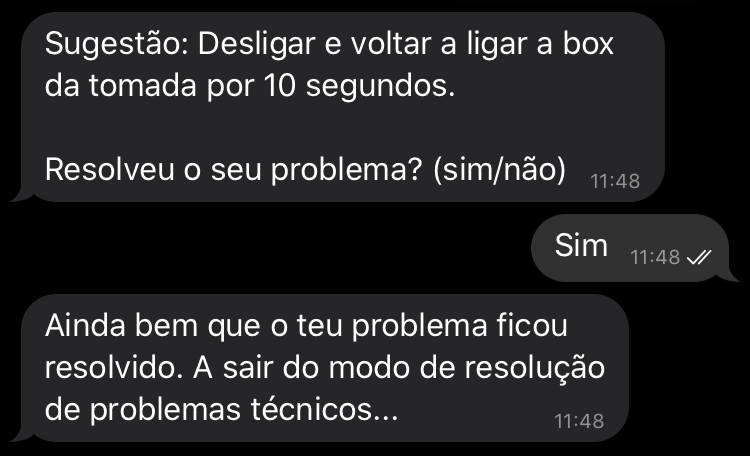
\includegraphics[width=4cm]{images/guiaoR/16_2.png}}}
    \end{figure}
\end{enumerate}

\end{appendices}

\end{document}